% Chapter Template

\chapter{Wstęp} % Main chapter title

\label{Chapter1} % Change X to a consecutive number; for referencing this chapter elsewhere, use \ref{ChapterX}

%----------------------------------------------------------------------------------------
%	SECTION 1
%----------------------------------------------------------------------------------------

\section{Opis}

Czosnek niedźwiedzi (Allium ursinum L.) – gatunek rośliny z podrodziny czosnkowych z rodziny amarylkowatych. Rośnie dziko w runie wilgotnych lasów liściastych, często w postaci rozległych łanów. Występuje na terenie Europy, na wschodzie po Ural i Kaukaz, w Europie jest też uprawiany. W Polsce częsty na południu, rzadszy na północy – na stanowiskach naturalnych objęty jest ochroną częściową. Gatunek wykorzystywany jest od dawna jako roślina jadalna, lecznicza i ozdobna. Ma właściwości lecznicze podobne do czosnku pospolitego, a przy tym wyróżnia się atrakcyjnym ulistnieniem i kwiatami. Jadalne są wszystkie części rośliny.

%-----------------------------------
%	SUBSECTION 1
%-----------------------------------
\section{Rozmieszczenie geograficzne}

Gatunek o zasięgu obejmującym rozległe obszary Europy. Na zachodzie występuje od Wysp Brytyjskich, Francji i Pirenejów, z nielicznymi stanowiskami na Półwyspie Iberyjskim, na północy sięga po równoleżnik 64° N w Norwegii i 60° 30' N w Finlandii. Na południu zasięg obejmuje południową Francję (w tym Korsykę), Włochy (w tym Sycylię), północną Grecję. W Europie Wschodniej rośnie w rozproszeniu w Krajach Nadbałtyckich, na Białorusi, na Ukrainie i w zachodniej Rosji. Izolowane, pojedyncze stanowiska wysunięte najdalej na wschód ma w paśmie środkowym gór Ural. Licznie rośnie w zachodnim Kaukazie, bardzo rzadki jest na Przedkaukaziu i w Azji Mniejszej.

Obszar, w którym czosnek występuje najobficiej, znajdując optymalne warunki rozwoju obejmuje zachodnie Niemcy, kraje Beneluxu i przyległe rejony Francji.

W Polsce spotykany jest na całym terenie, głównie jednak w Sudetach, Karpatach, na Pogórzu i na przyległych wyżynach, gdzie jest dość pospolity. Na niżu występuje na bardzo rozproszonych stanowiskach, zwłaszcza rzadki jest w obszarze od Ziemi Lubuskiej, przez Wielkopolskę, Mazowsze po Podlasie. Rośnie nieco częściej w obrębie pojezierzy pomorskich i mazurskich.

Nie rośnie w górach powyżej 1900 m n.p.m. W Polsce najczęściej na wysokościach między 300 i 700 m n.p.m., najwyżej na wysokości 1150 m n.p.m. na stokach Babiej Góry.

%-----------------------------------
%	SUBSECTION 2
%-----------------------------------

\section{Morfologia}
\subsection{Pokrój}
Roślina osiąga wysokość 20–50 cm. Rośnie w płatach, czasami tworzy duże, zwarte łany.

\begin{figure}
 \centering
 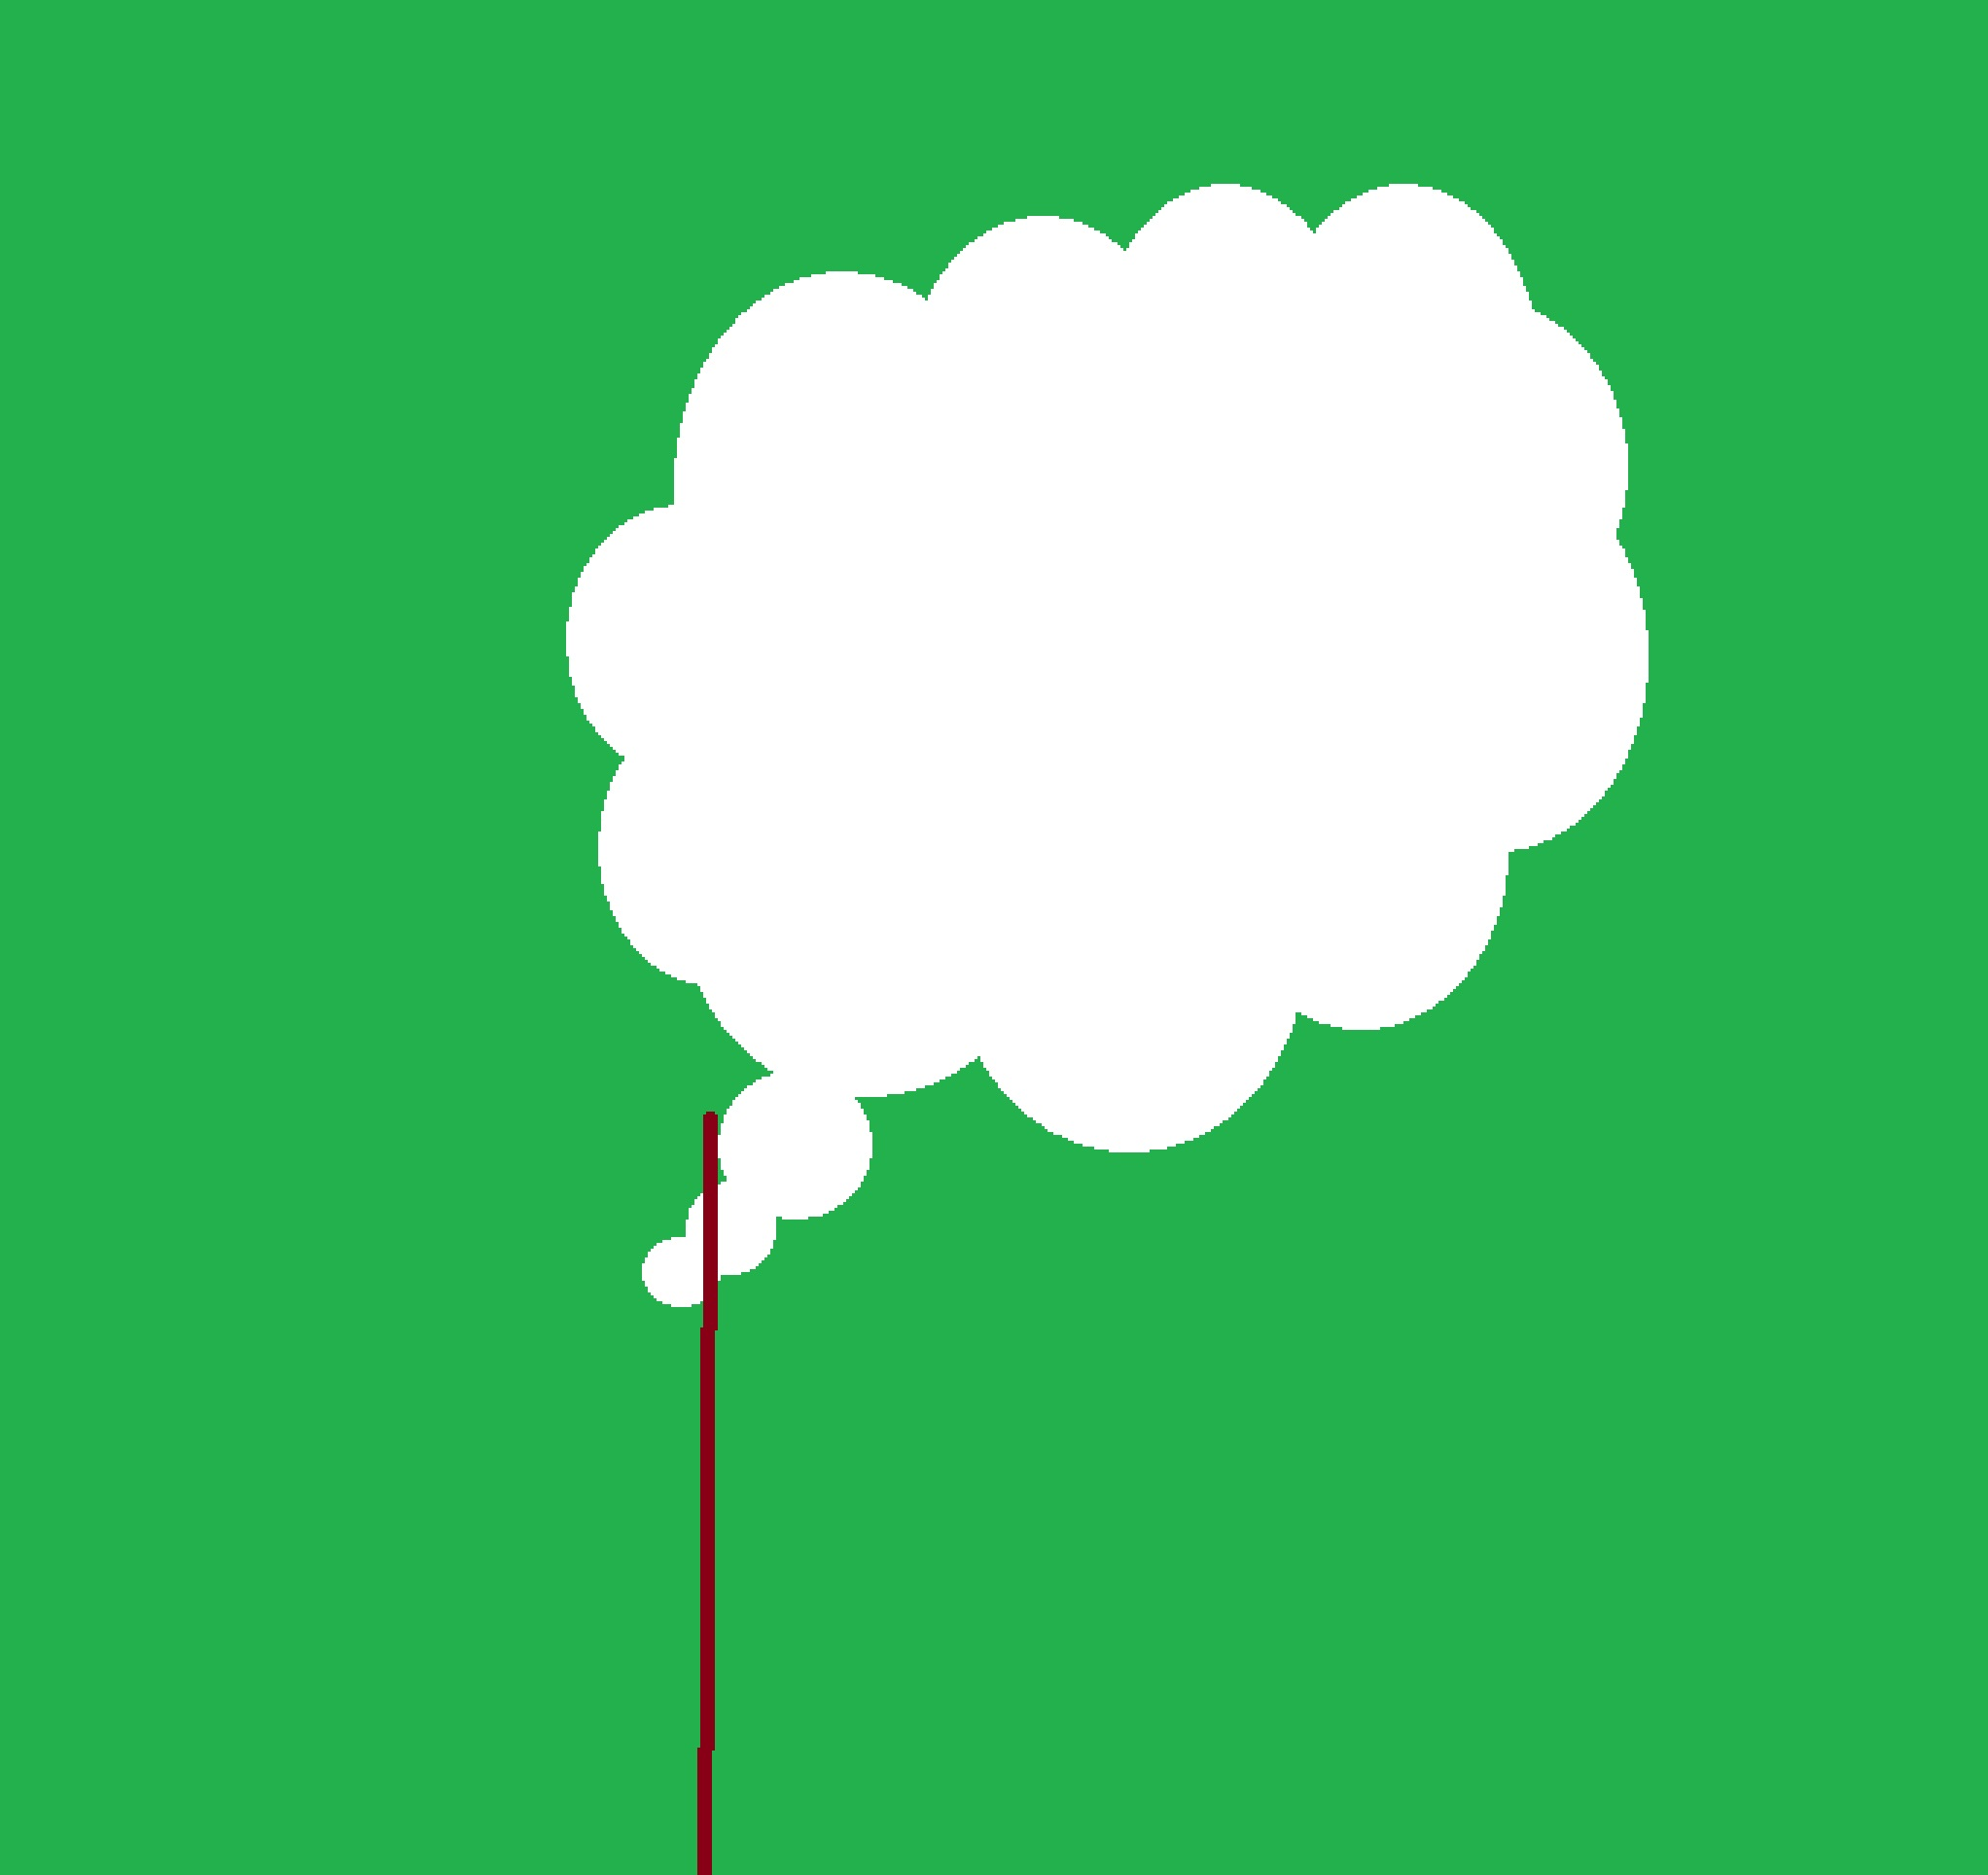
\includegraphics[height=3cm]{czosnek.jpg}
 \caption{Herb i godło Politechniki Gdańskiej\\
a) herb obowiązujący do 30 września 2013 r., b) godło obowiązujące od 1 października 2013 r., w polskiej wersji językowej, c) godło obowiązujące od 1 października 2013 r., w angielskiej wersji językowej}
 \label{figure:example}
\end{figure}

\begin{figure}
 \centering
 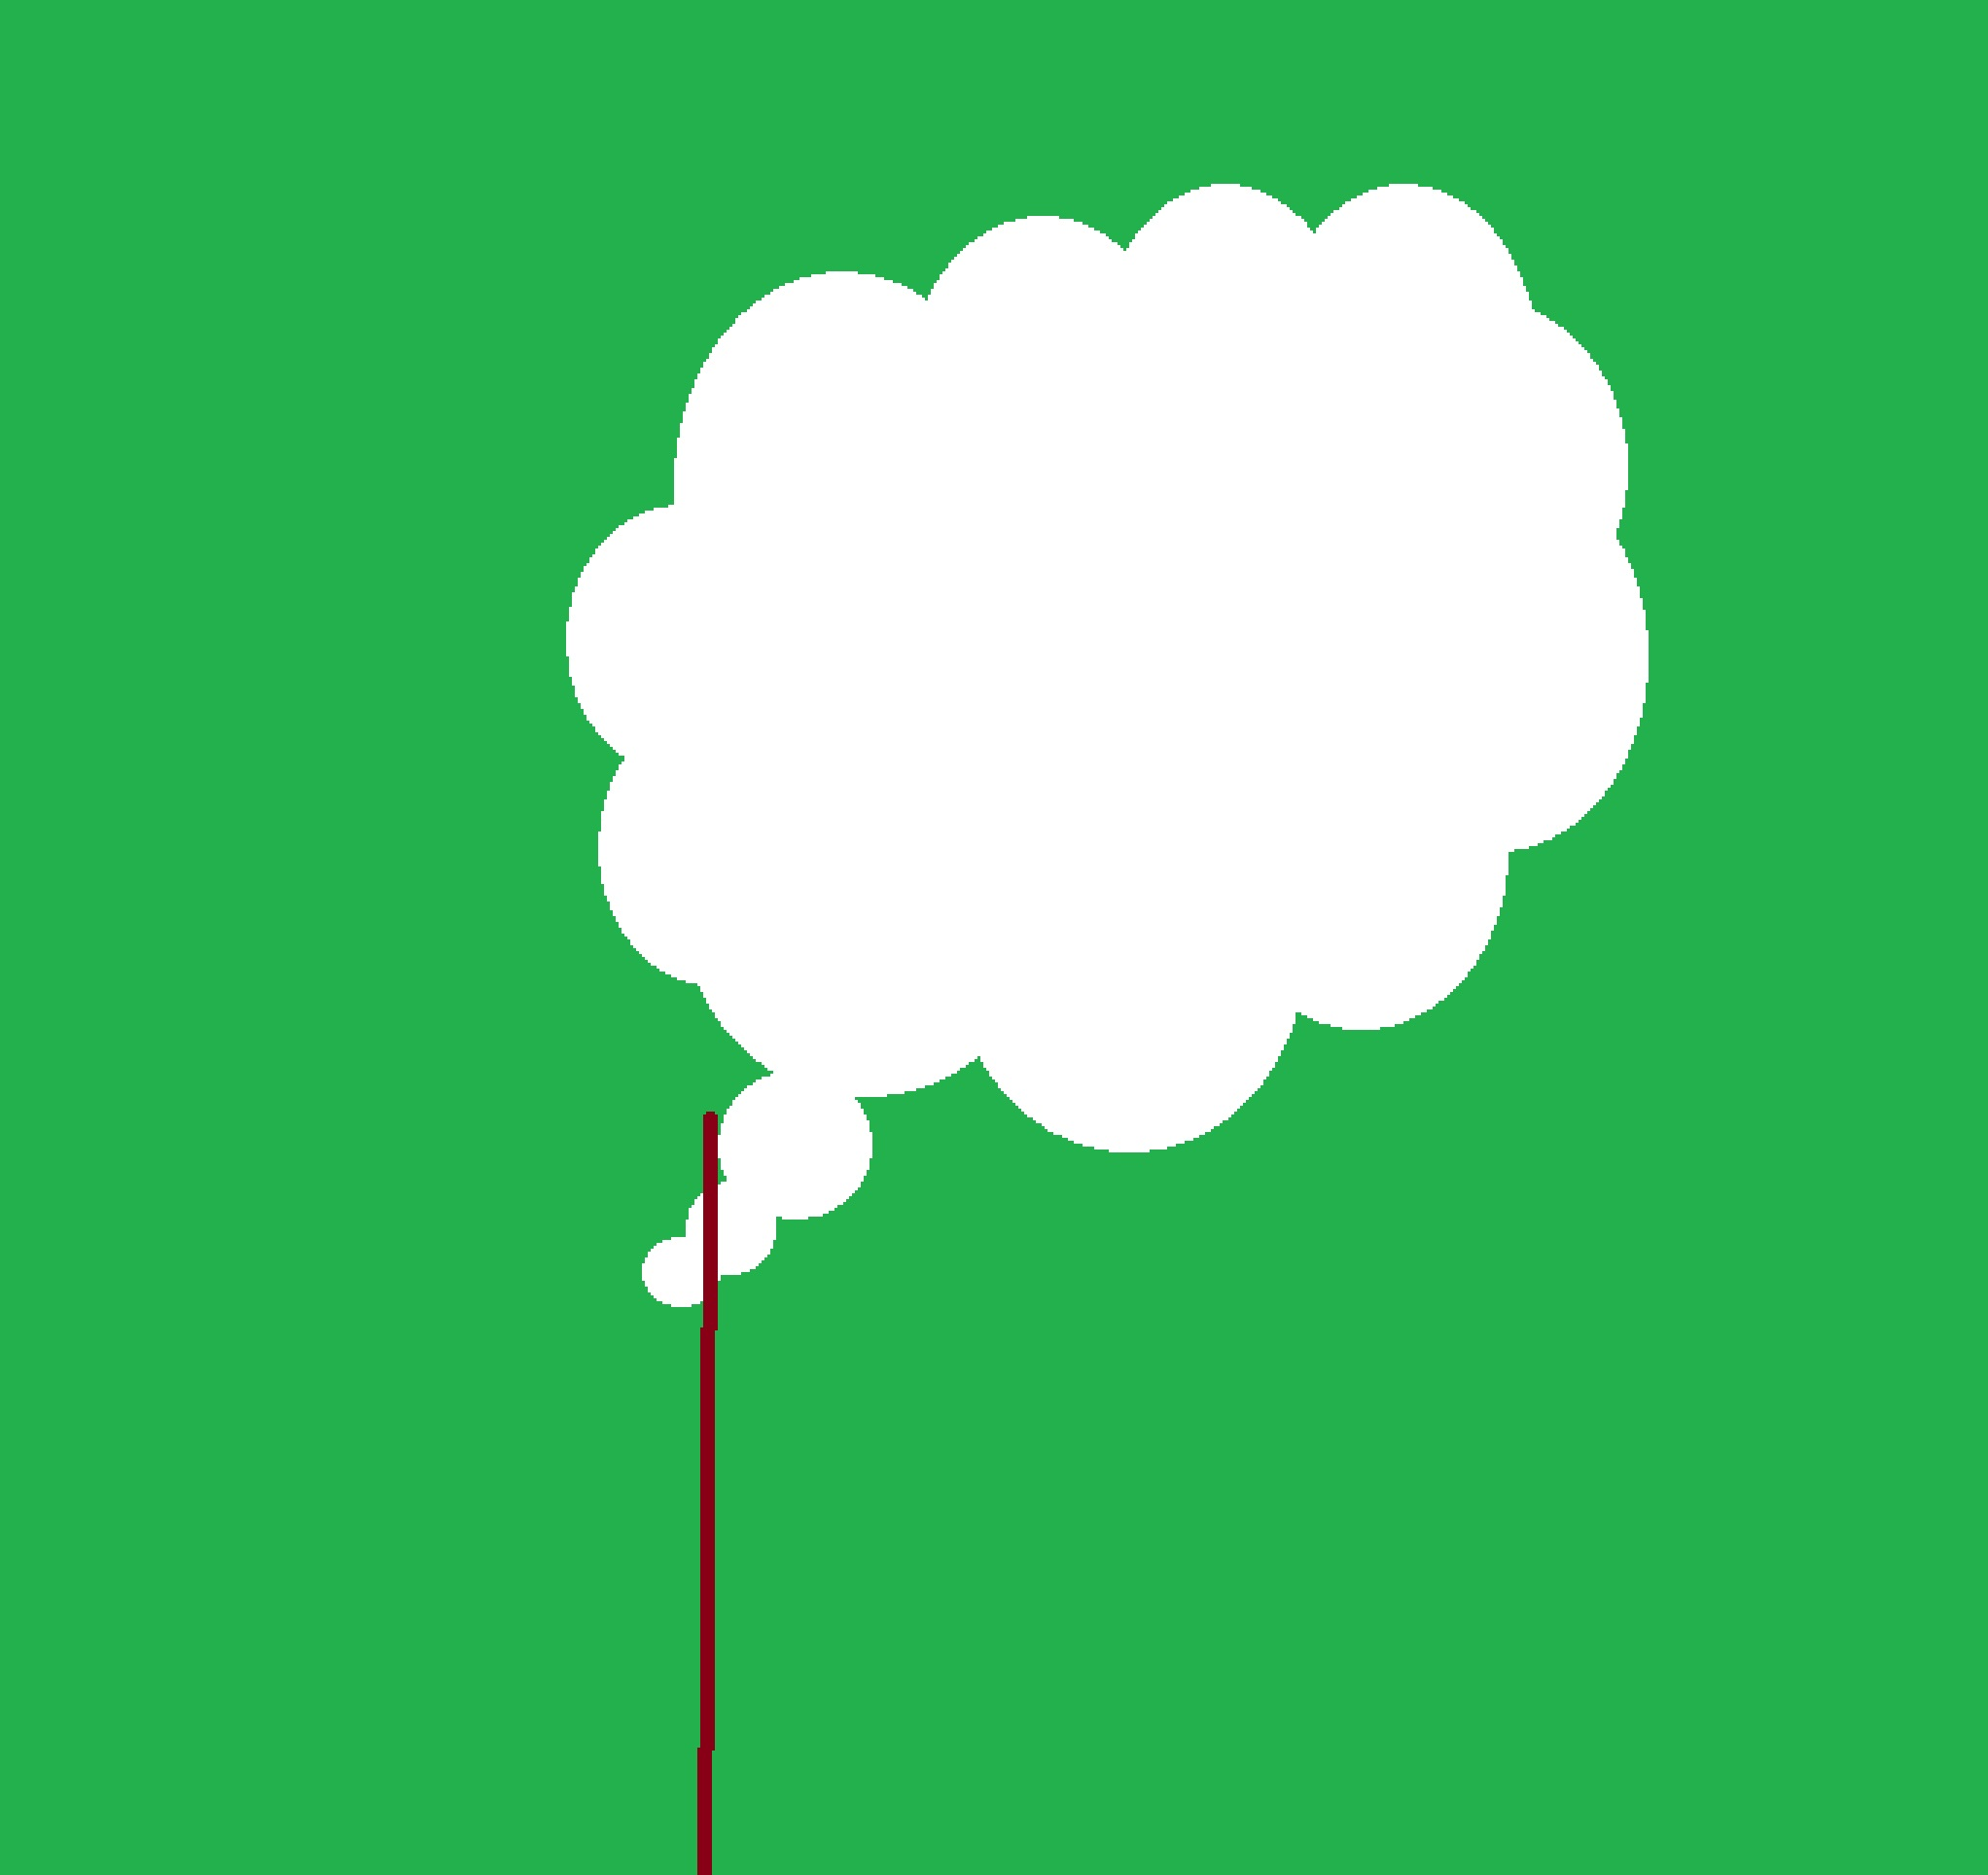
\includegraphics[height=3cm]{czosnek.jpg}
 \caption{Obraz numer 2}
 \label{figure:example1}
\end{figure}

\subsection{Organy podziemne}
Cebula wąska, długa na 1,5–5,5 cm (najczęściej 2–4,5 cm); stanowi zgrubiałą nasadę ogonka liściowego górnego liścia. U silnie rosnących roślin powstają czasem w ciągu sezonu dwie cebule z nabrzmiałych ogonków dwóch górnych liści. Młoda cebula na początku roku jest gładka, z nielicznymi włóknami u nasady. Rozwój potomnej cebuli powoduje zamianę starej w postrzępioną masę włóknistą, co następuje w czasie kwitnienia. W dolnej części cebuli spichrzowa część ogonka liściowego otacza bardzo skrócony pęd. Z jego dolnego końca wyrasta kilka (zwykle do 10) cienkich korzeni płytko rozrastających się mniej więcej poziomo w warstwie przypowierzchniowej gleby (do 3 cm głębokości), oraz 2–3 tęższe korzenie kurczliwe rosnące niemal pionowo w dół. Te ostatnie mają za zadanie wciąganie cebuli w głąb podłoża, i często na końcach są nieco zgrubiałe. Wszystkie korzenie są słabo rozgałęzione i osiągają do ok. 30 cm długości.

\subsection{Liście}
Pierwszy liść rozwija się po przeciwnej stronie pędu w stosunku do szypuły kwiatostanowej wyrastającej w poprzednim sezonie wegetacyjnym. Tworzy niewielką, bezbarwną pochwę, chroniącą kolejne liście podczas ich wzrostu przez glebę. Z jego kąta wyrasta też pęd kwiatostanowy. Liście asymilacyjne są odziomkowe, zazwyczaj dwa, czasem trzy lub jeden. Długoogonkowe, z blaszką kształtu eliptyczno-lancetowatego, zaostrzoną na końcu i zbiegającą u nasady, długą na ok. 25 cm, szeroką na 2–6 cm, płaską, cienką, o soczyście zielonej barwie. Ogonki są skręcone w części podziemnej, w wyniku czego morfologicznie dolna, ciemniejsza powierzchnia liści skierowana jest ku górze.

%----------------------------------------------------------------------------------------
%	SECTION 2
%----------------------------------------------------------------------------------------

\section{Biologia}
\subsection{Rozwój}
Bylina, geofit cebulowy. Wzrost korzeni jest najbardziej intensywny jesienią i na początku wiosny. Nowe liście pojawiają się nad ziemią między końcem lutego a początkiem kwietnia (w zależności od warunków klimatycznych). Dzięki temu roślina korzystać może z dostatecznej ilości światła wobec braku listowia w warstwie koron drzew. Z kolei późną wiosną rozwijające się liście drzew chronią czosnek przed nadmiernym nasłonecznieniem i zapewniają odpowiednie warunki wilgotnościowe na dnie lasu. Czosnek niedźwiedzi kwitnie od kwietnia do czerwca, najintensywniej w maju. Kwiaty zapylane są przez trzmiele i muchy. Jednak gdy nie dojdzie do zapylenia krzyżowego, co zdarza się prawdopodobnie często, następuje samozapylenie – niezapylony słupek wygina się dotykając pręcików. Dzięki temu dochodzi do zapłodnienia i wytworzenia nasion również wtedy, gdy kwiatów nie odwiedziły owady. Owoce i nasiona dojrzewają w czerwcu i lipcu, nieco później u roślin rosnących na wystawie północnej, albo w latach chłodniejszych. Wraz z nadejściem lata nadziemne części roślin w krótkim czasie więdną i obumierają, przy czym w miejscach wilgotnych pozostają zielone 2–3 tygodnie dłużej.
\begin{figure}[ht]
 \centering
 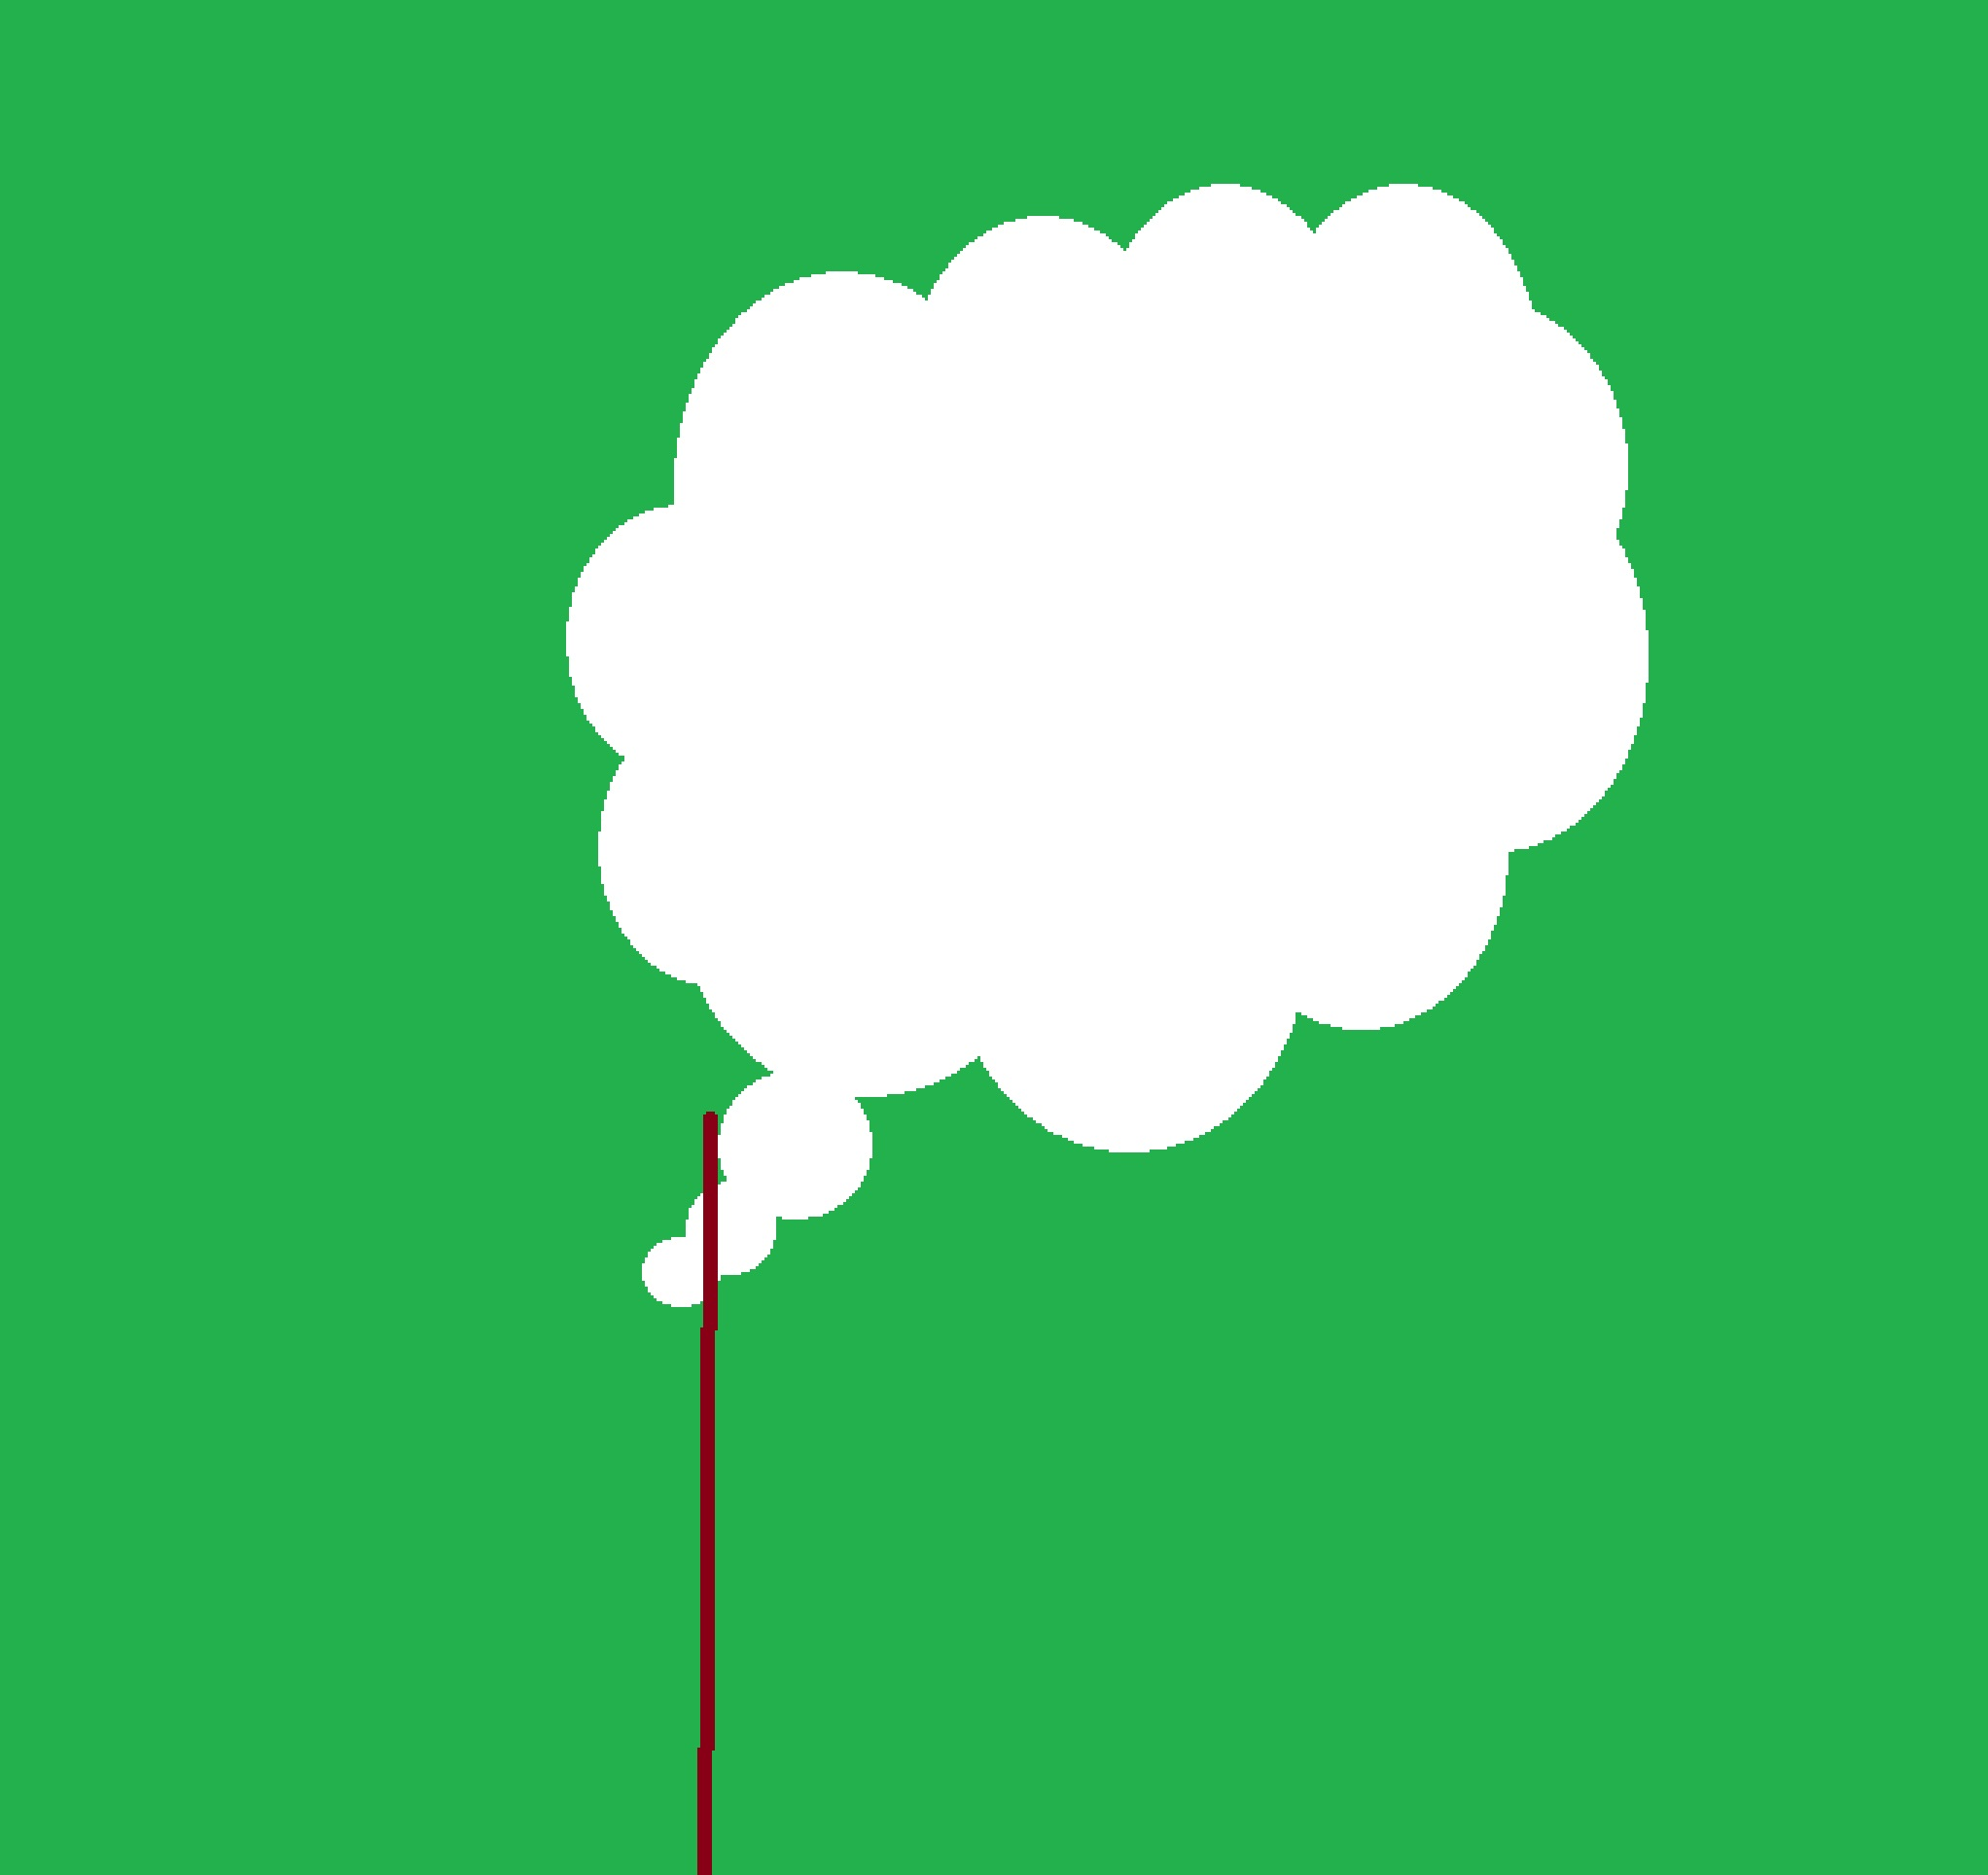
\includegraphics[height=3cm]{czosnek.jpg}
 \caption{Obraz numer 10}
 \label{figure10}
\end{figure}

Nasiona w większości spadają w bezpośrednim sąsiedztwie rośliny macierzystej. W łupinie nasiennej mają zgromadzony tłuszcz tworzący elajosom i z tego powodu niektóre źródła stwierdzają, że stanowi on pożywienie mrówek przyczyniających się do transportu nasion (myrmekochoria). W istocie jednak mrówki nie przenoszą diaspor czosnku. Transportowane są one wraz z cząstkami gleby przylepiającymi się do kończyn zwierząt i człowieka. Ponieważ zdarza się to rzadko i większość nasion kiełkuje w pobliżu rośliny macierzystej – gatunek ma specyficznie chaotyczny, płatowy typ rozmieszczenia.

\begin{equation} \label{mc2}
E = mc^2
\end{equation}
\begin{equation} \label{beta}
\beta = \omega\sqrt{\mu\varepsilon}
\end{equation}
Z równania \eqref{mc2} i \eqref{beta}, po kilku prostych przekształceniach, otrzymujemy równanie \eqref{kkk}.
\begin{equation} \label{kkk}
\beta = \frac{\omega}{c}
\end{equation}

\begin{equation} \label{test}
\boldmath
 z = \overbrace{
   \underbrace{x}_\text{real} + i
   \underbrace{y}_\text{imaginary}
  }^\text{complex number}
\end{equation}

Nasiona bywają także transportowane przez wodę, co może odgrywać istotną rolę w lasach zalewowych. Kiełkują zwykle dopiero po 14 miesiącach, rzadko w tym samym roku (od listopada do kwietnia). Zarodek jest krótki i niemal prosty. Kiełkowanie jest hipogeiczne. Liścień jest cylindryczny, podobnie kolejne 1-2 liście, szybko odpadające. Kolejny liść ma wąską blaszkę liściową, a nasada jego ogonka tworzy pierwszą, niewielką cebulkę. Śmiertelność w ciągu pierwszych dwóch lat życia wynosi 21\%. W drugim lub trzecim roku rozwijają się korzenie kurczliwe (rosnące pionowo, wciągające cebulę w głąb gleby) i roślina w większym stopniu narażona jest na atak nicieni i owadów. W sumie wiek reprodukcyjny osiąga od 1 do 10\% siewek. Kwitnąć zaczynają rośliny w wieku 3 lub 4–5 lat. Później kwitnienie i owocowanie jest już coroczne, o ile warunki siedliskowe na to pozwalają. Cebule wciągane przez korzenie kurczliwe u dziesięcioletnich roślin rosnących w bardzo pulchnej glebie znajdowane były na głębokości do 27 cm.

\begin{figure}[ht]
 \centering
 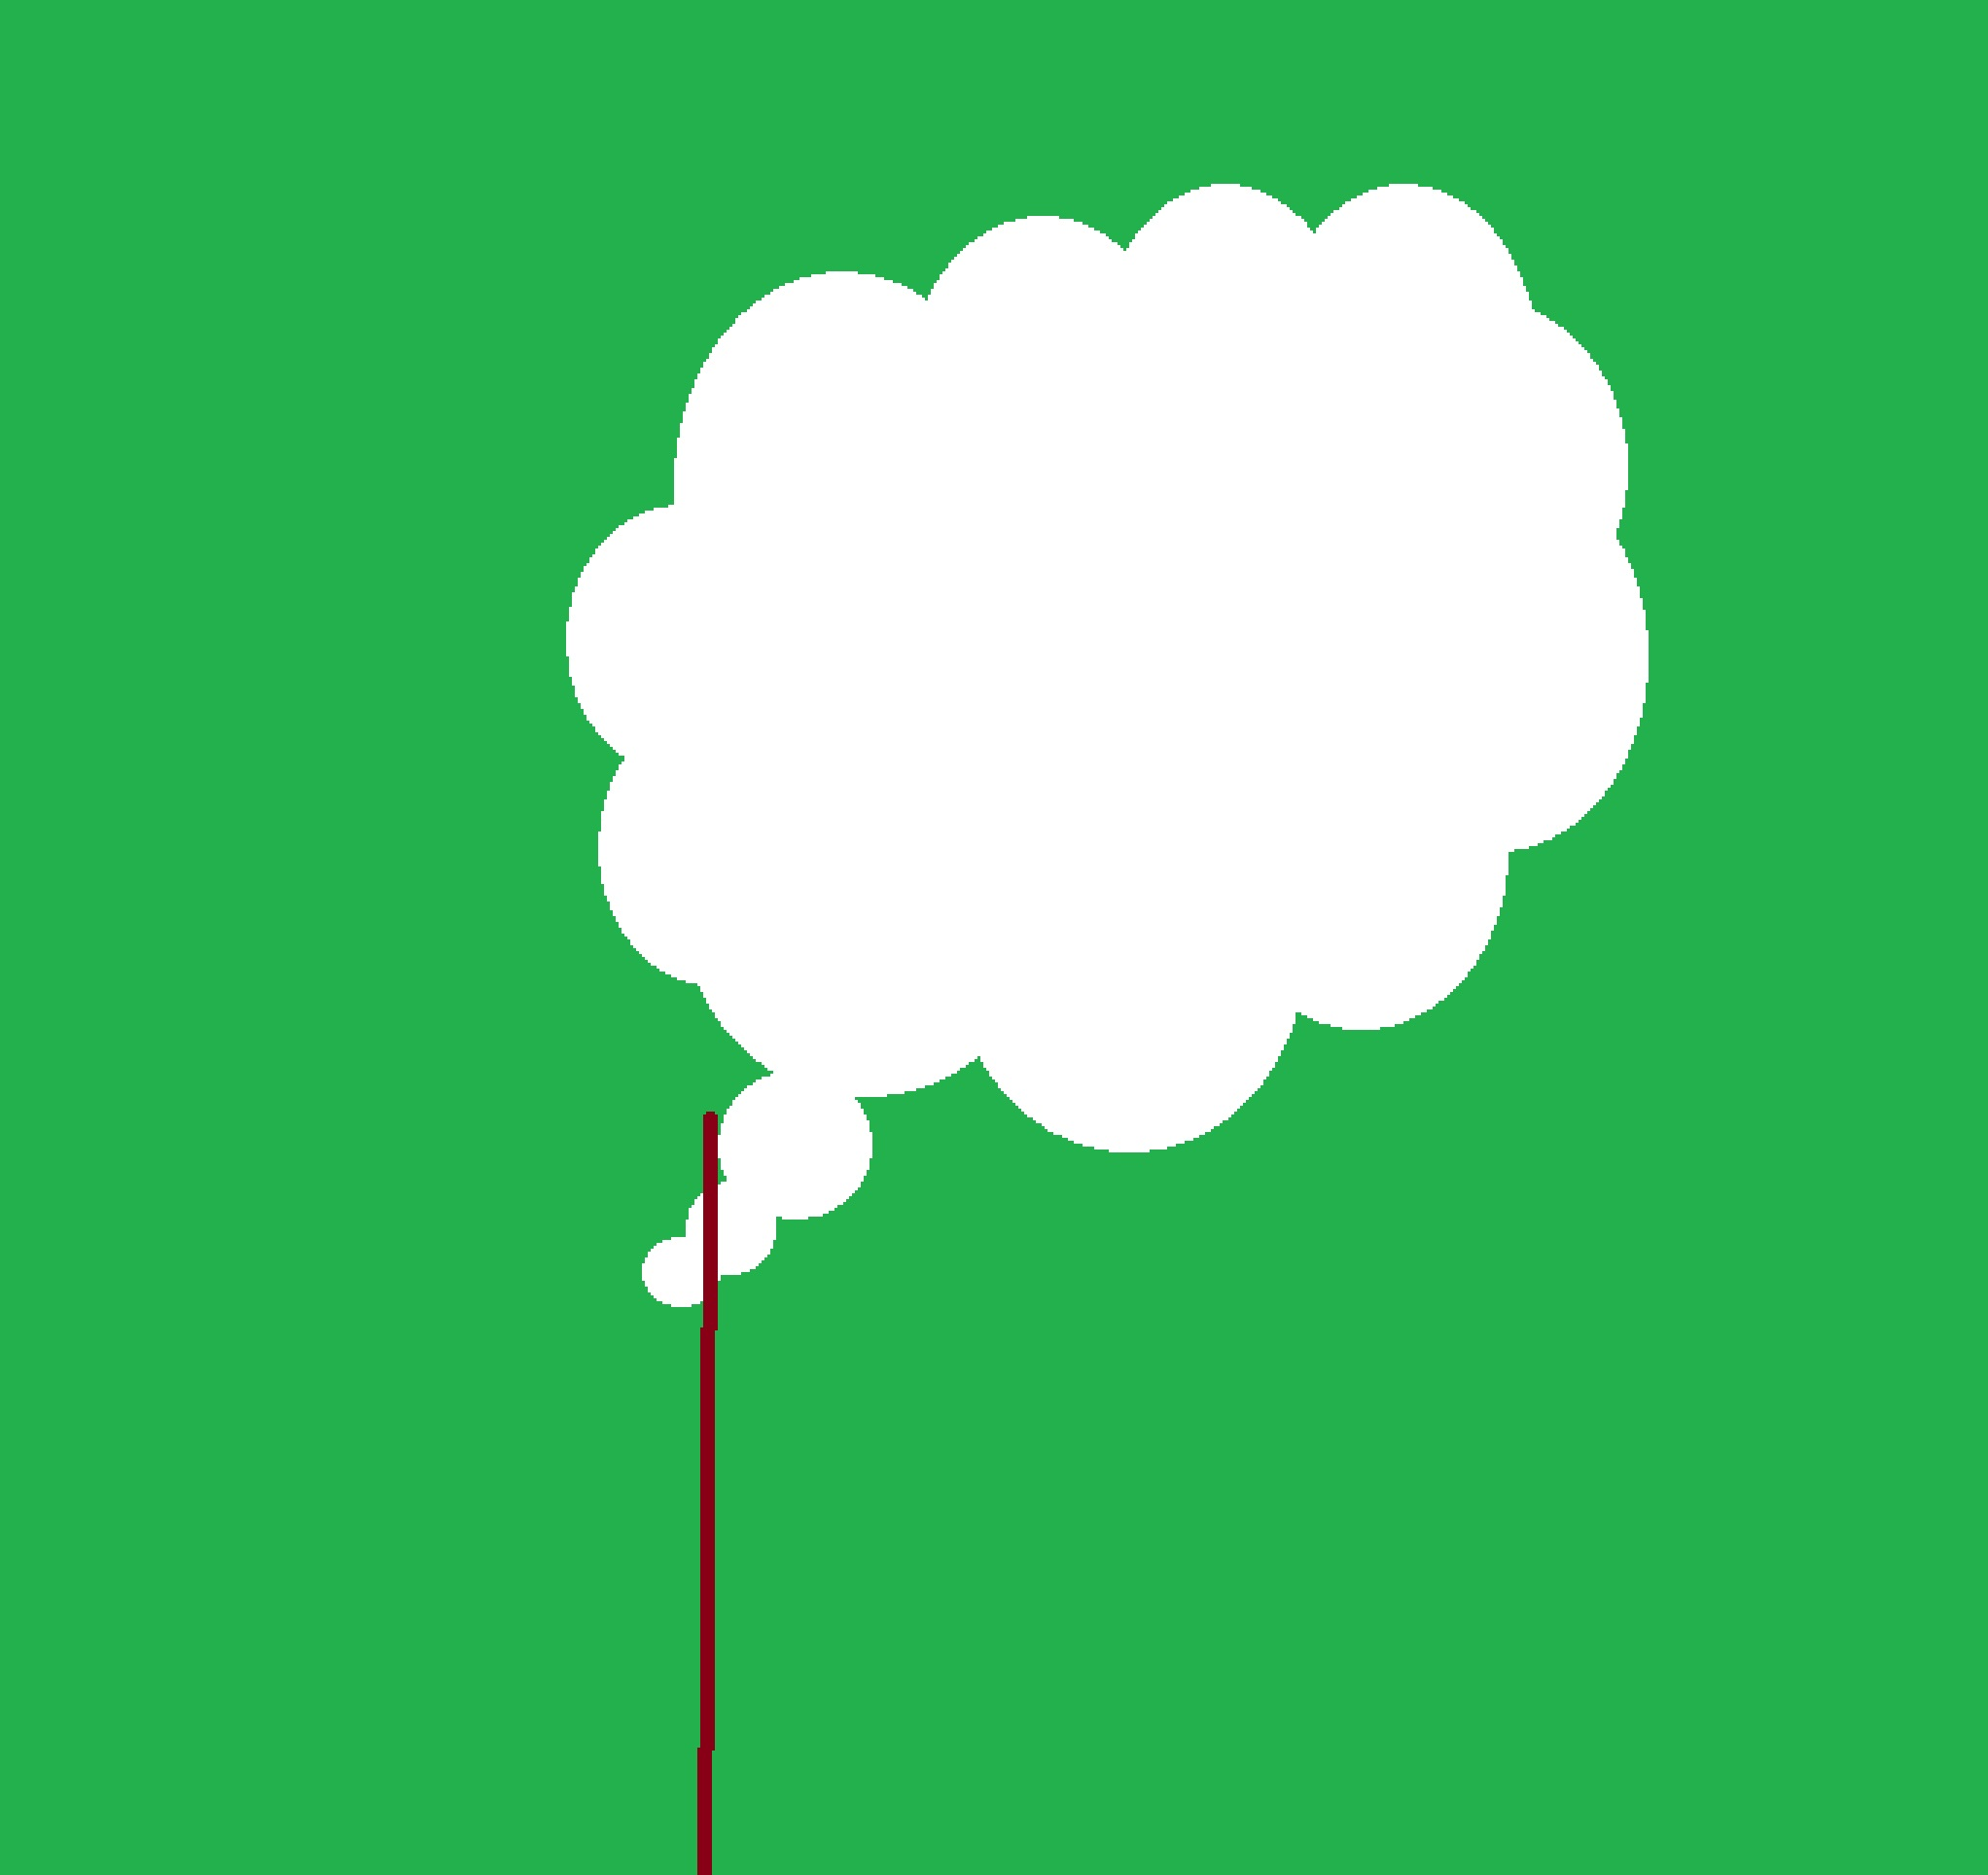
\includegraphics[height=3cm]{czosnek.jpg}
 \caption{Obraz numer 3}
 \label{figure3}
\end{figure}

\begin{figure}
 \centering
 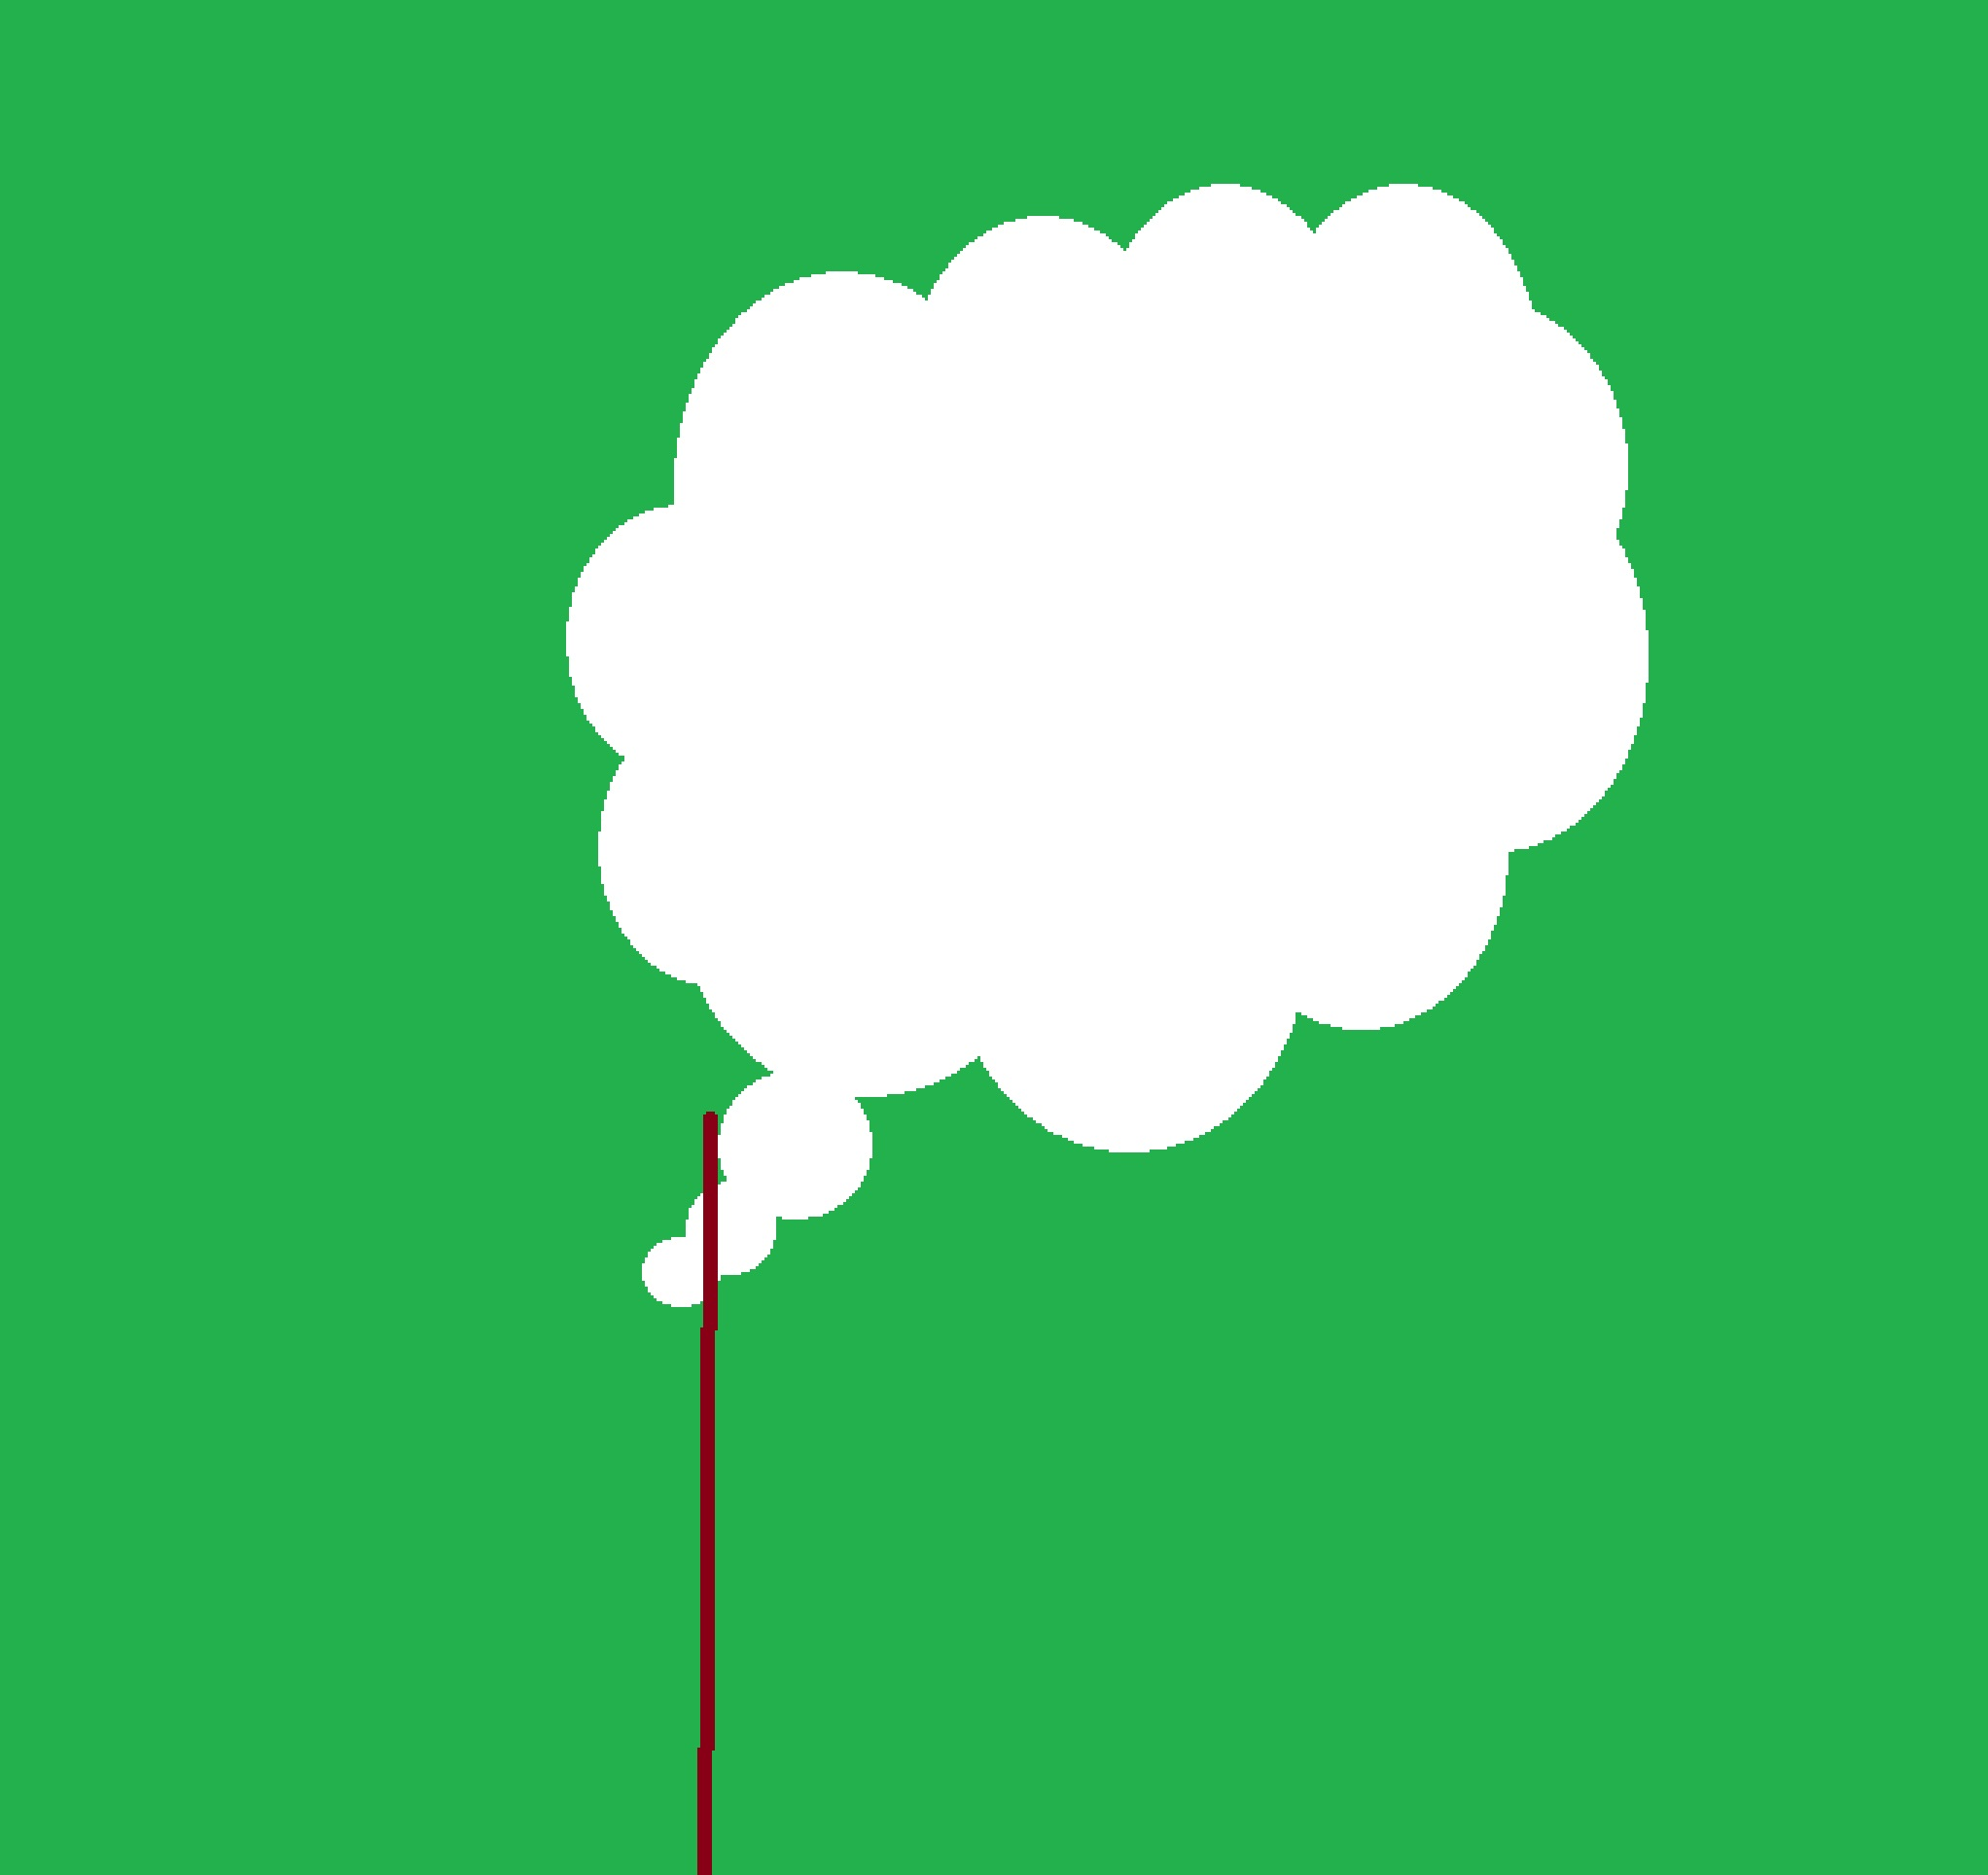
\includegraphics[height=3cm]{czosnek.jpg}
 \caption{Obraz numer 9}
 \label{figure:example2}
\end{figure}

Roślina rozmnaża się głównie przez nasiona. Tylko u silnie rosnących roślin, u których w jednym sezonie rozwijają się trzy liście – powstać mogą dwie cebule potomne. Rośliny starzeją się i przestają kwitnąć w wieku lat 7–8. Maksymalny czas życia poszczególnych roślin wynosi 8–10 lat, przy czym występują jeszcze trzy wcześniejsze fazy zamierania roślin: w fazie zarodkowej, w wyniku autolizy nasion w okresie ich spoczynku, podczas wciągania cebuli w głębsze warstwy gleby przez korzenie kurczliwe.

\begin{figure}
 \centering
 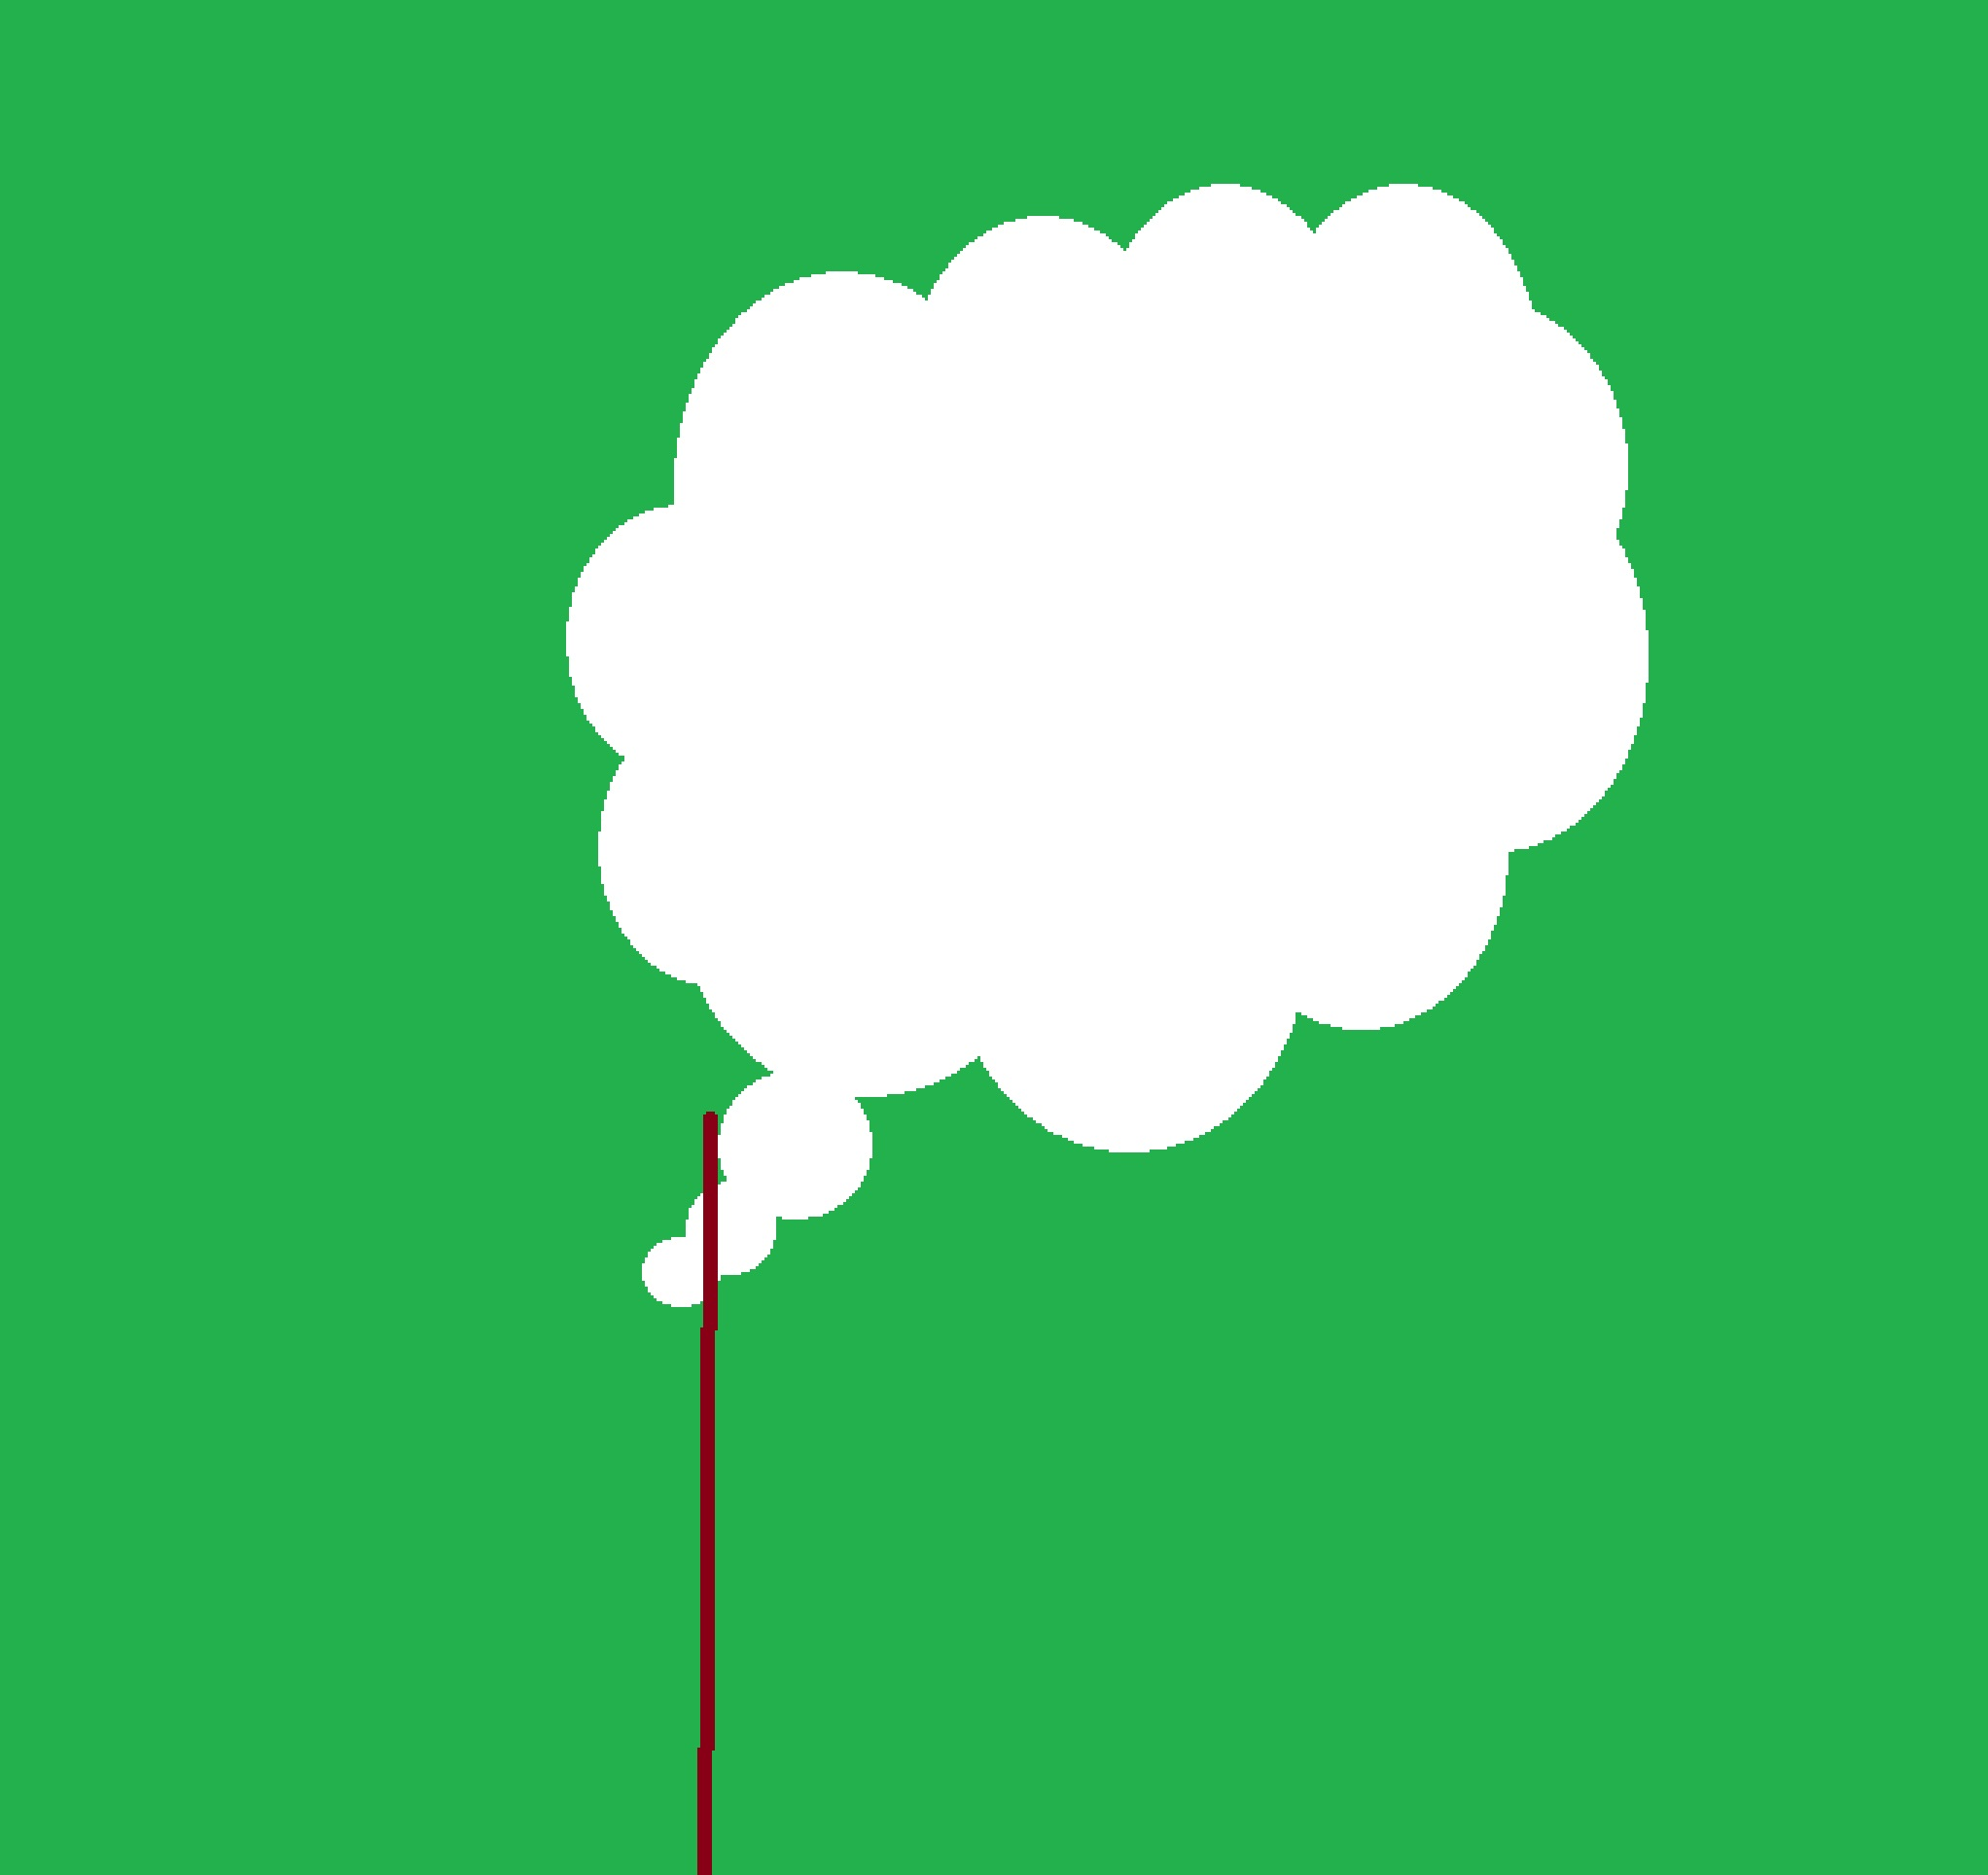
\includegraphics[height=3cm]{czosnek.jpg}
 \caption{Obraz numer 8}
 \label{figure:example3}
\end{figure}

Czosnek niedźwiedzi rośnie w dużych zagęszczeniach, często na rozległych powierzchniach. Na 1 m2 w obrębie stanowiska naliczono ponad 1900 małych roślin, 331 średnich i 63 duże rośliny, przy czym większość z nich uznano za wyrosłe z nasion. Na 1 m2 przy 156 owocujących baldachach zarejestrowano powstanie ponad 9 tys. nasion, a maksymalnie udokumentowano wytwarzanie 10 tys. nasion przez rośliny rosnące na 1 m2. Średnio na jednym ze stanowisk powstawały 2692 nasiona na 1 m2.

\subsection{Cechy fitochemiczne}
Cała roślina wydziela silny, charakterystyczny czosnkowy zapach. Ziele zawiera do 0,007\% olejku eterycznego (zwanego ursaliną), którego składniki – siarczki i wielosiarczki alkilowe – odpowiadają za specyficzny aromat. Gatunek należy do grupy czosnków, w których głównymi związkami tej grupy są alliina i methiina (metylo-alliina), mniejszą rolę odgrywają: isoalliina, propiina i ethiina. Poza tym olejek zawiera m.in. wielosiarczki dwuwinylowe i tiole. Skład chemiczny olejku jest bardzo zmienny w zależności od miejsca i czasu zbioru. W cebulach znajduje się od 2,7 do 7,7 mg% kwasu askorbinowego. Ziele zawiera także szereg flawonoidów glikozydowych, związków fenolowych, saponin steroidowych, lektyny, cebula obfituje w polisacharydy (zwłaszcza fruktany) i kwasy tłuszczowe (palmitynowy, oleopalmitynowy, linolowy, oleinowy, stearynowy, α-linolenowy i mirystynowy). Z makro- i mikroelementów czosnek niedźwiedzi wyróżnia się wysoką zawartością magnezu (7,0 mg/kg), manganu (1,6 mg/kg) i żelaza (230 mg/kg). Cechuje się także znaczną ilością adenozyny (120 mg/kg).

Olejek wydzielany przez rośliny rosnące w naturze zawiera tak wiele związków siarki, że to właśnie nad czosnkiem niedźwiedzim zarejestrowano największą emisję tego pierwiastka spośród wszystkich roślin.

Przynajmniej dla części ssaków jest to roślina trująca. Do bardzo wrażliwych na zatrucia tym gatunkiem należą psy.

\subsection{Genetyka}
Liczba chromosomów 2n=14. W Europie Zachodniej stwierdzono bardzo nikłe zróżnicowanie genetyczne nawet między odległymi populacjami.

\begin{figure}
 \centering
 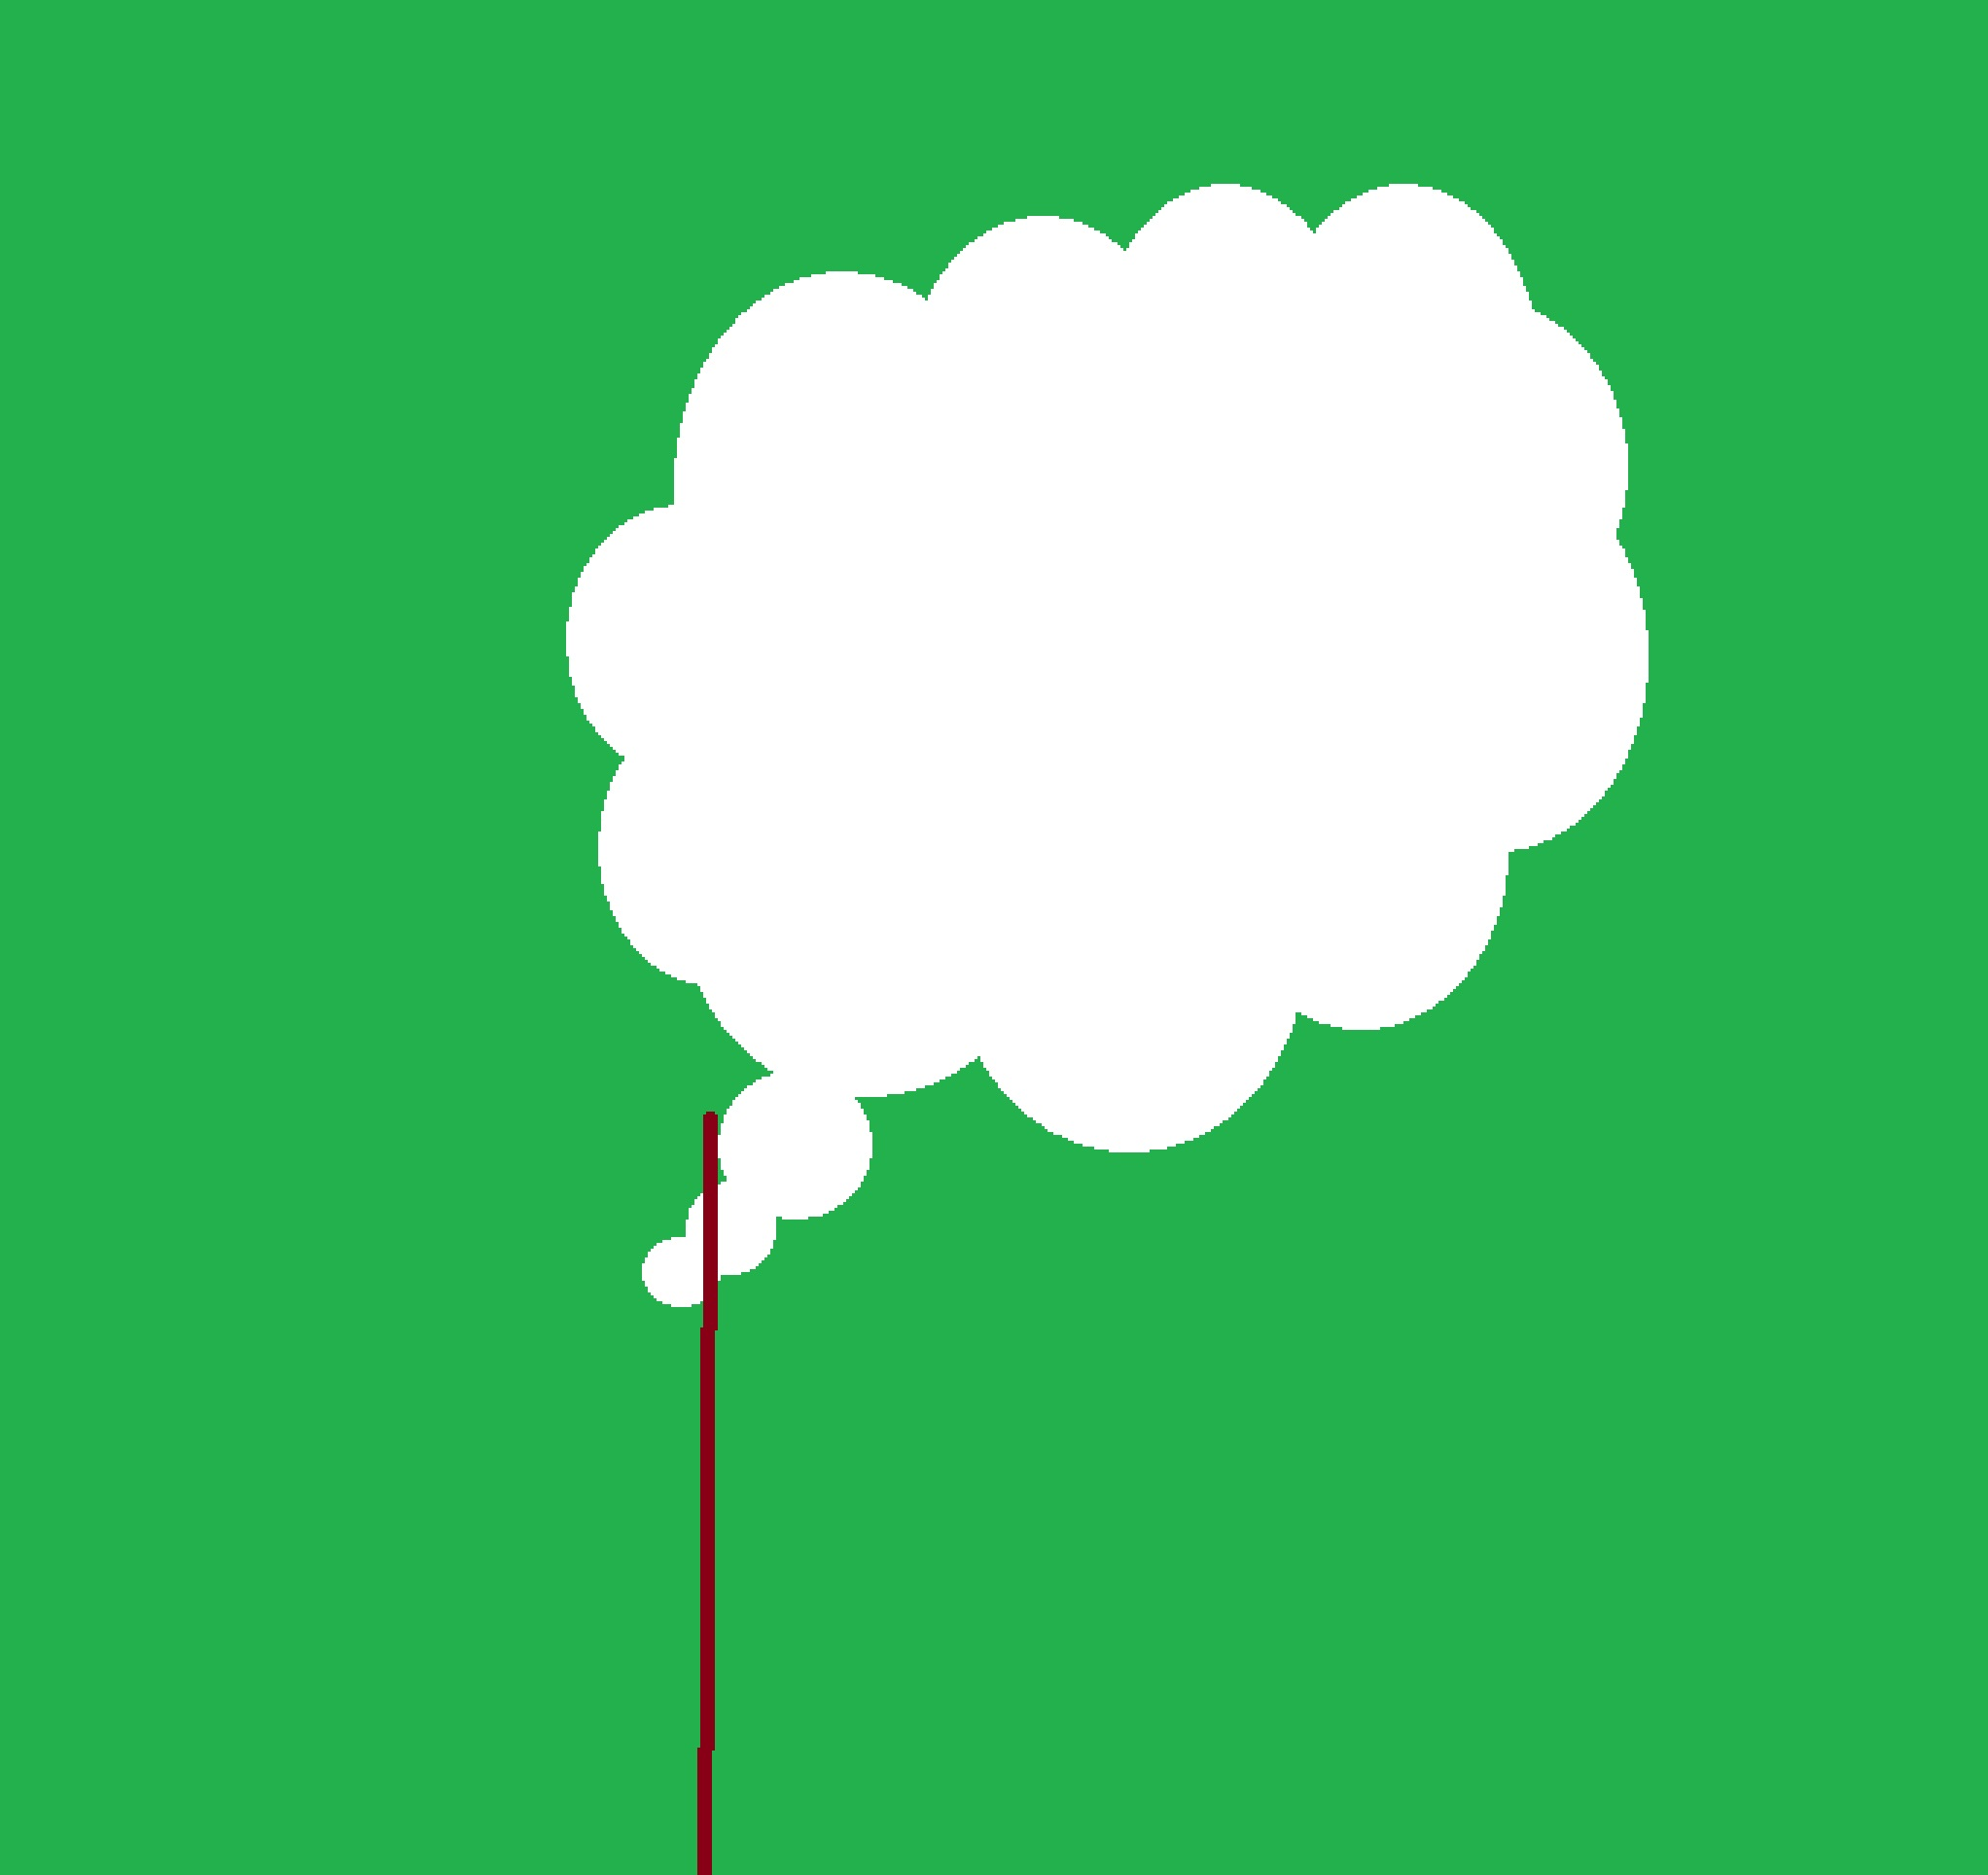
\includegraphics[height=3cm]{czosnek.jpg}
 \caption{Obraz numer 7}
 \label{figure:example4}
\end{figure}

\section{Ekologia}
\subsection{Siedlisko}
Rośnie zwykle w wilgotnych i cienistych lasach liściastych, poza lasami zdarza się w obszarach o wysokich i regularnych opadach. Preferuje gleby przepuszczalne, próchniczne, świeże, gliniasto-piaszczyste i gliniaste, zarówno zasobne w wapń, jak i ubogie w jego związki. Odczyn gleb w miejscach występowania gatunku wynosi od 5,5 do 7,9 pH. Nie rośnie na glebach piaszczystych, ubogich i w miejscach, w których stagnuje woda. Często zasiedla stoki wzniesień i dolin ze względu na łatwe odprowadzanie z nich wody. Unika gleb z wysoką koncentracją glinu (pierwiastek ten w wyższych stężeniach blokuje rozwój korzeni czosnku). W warunkach bardzo silnego zacienienia rośliny rosną słabiej i nie zakwitają. Silne nasłonecznienie i susza z kolei powodują ich szybkie więdnięcie.

\begin{figure}
 \centering
 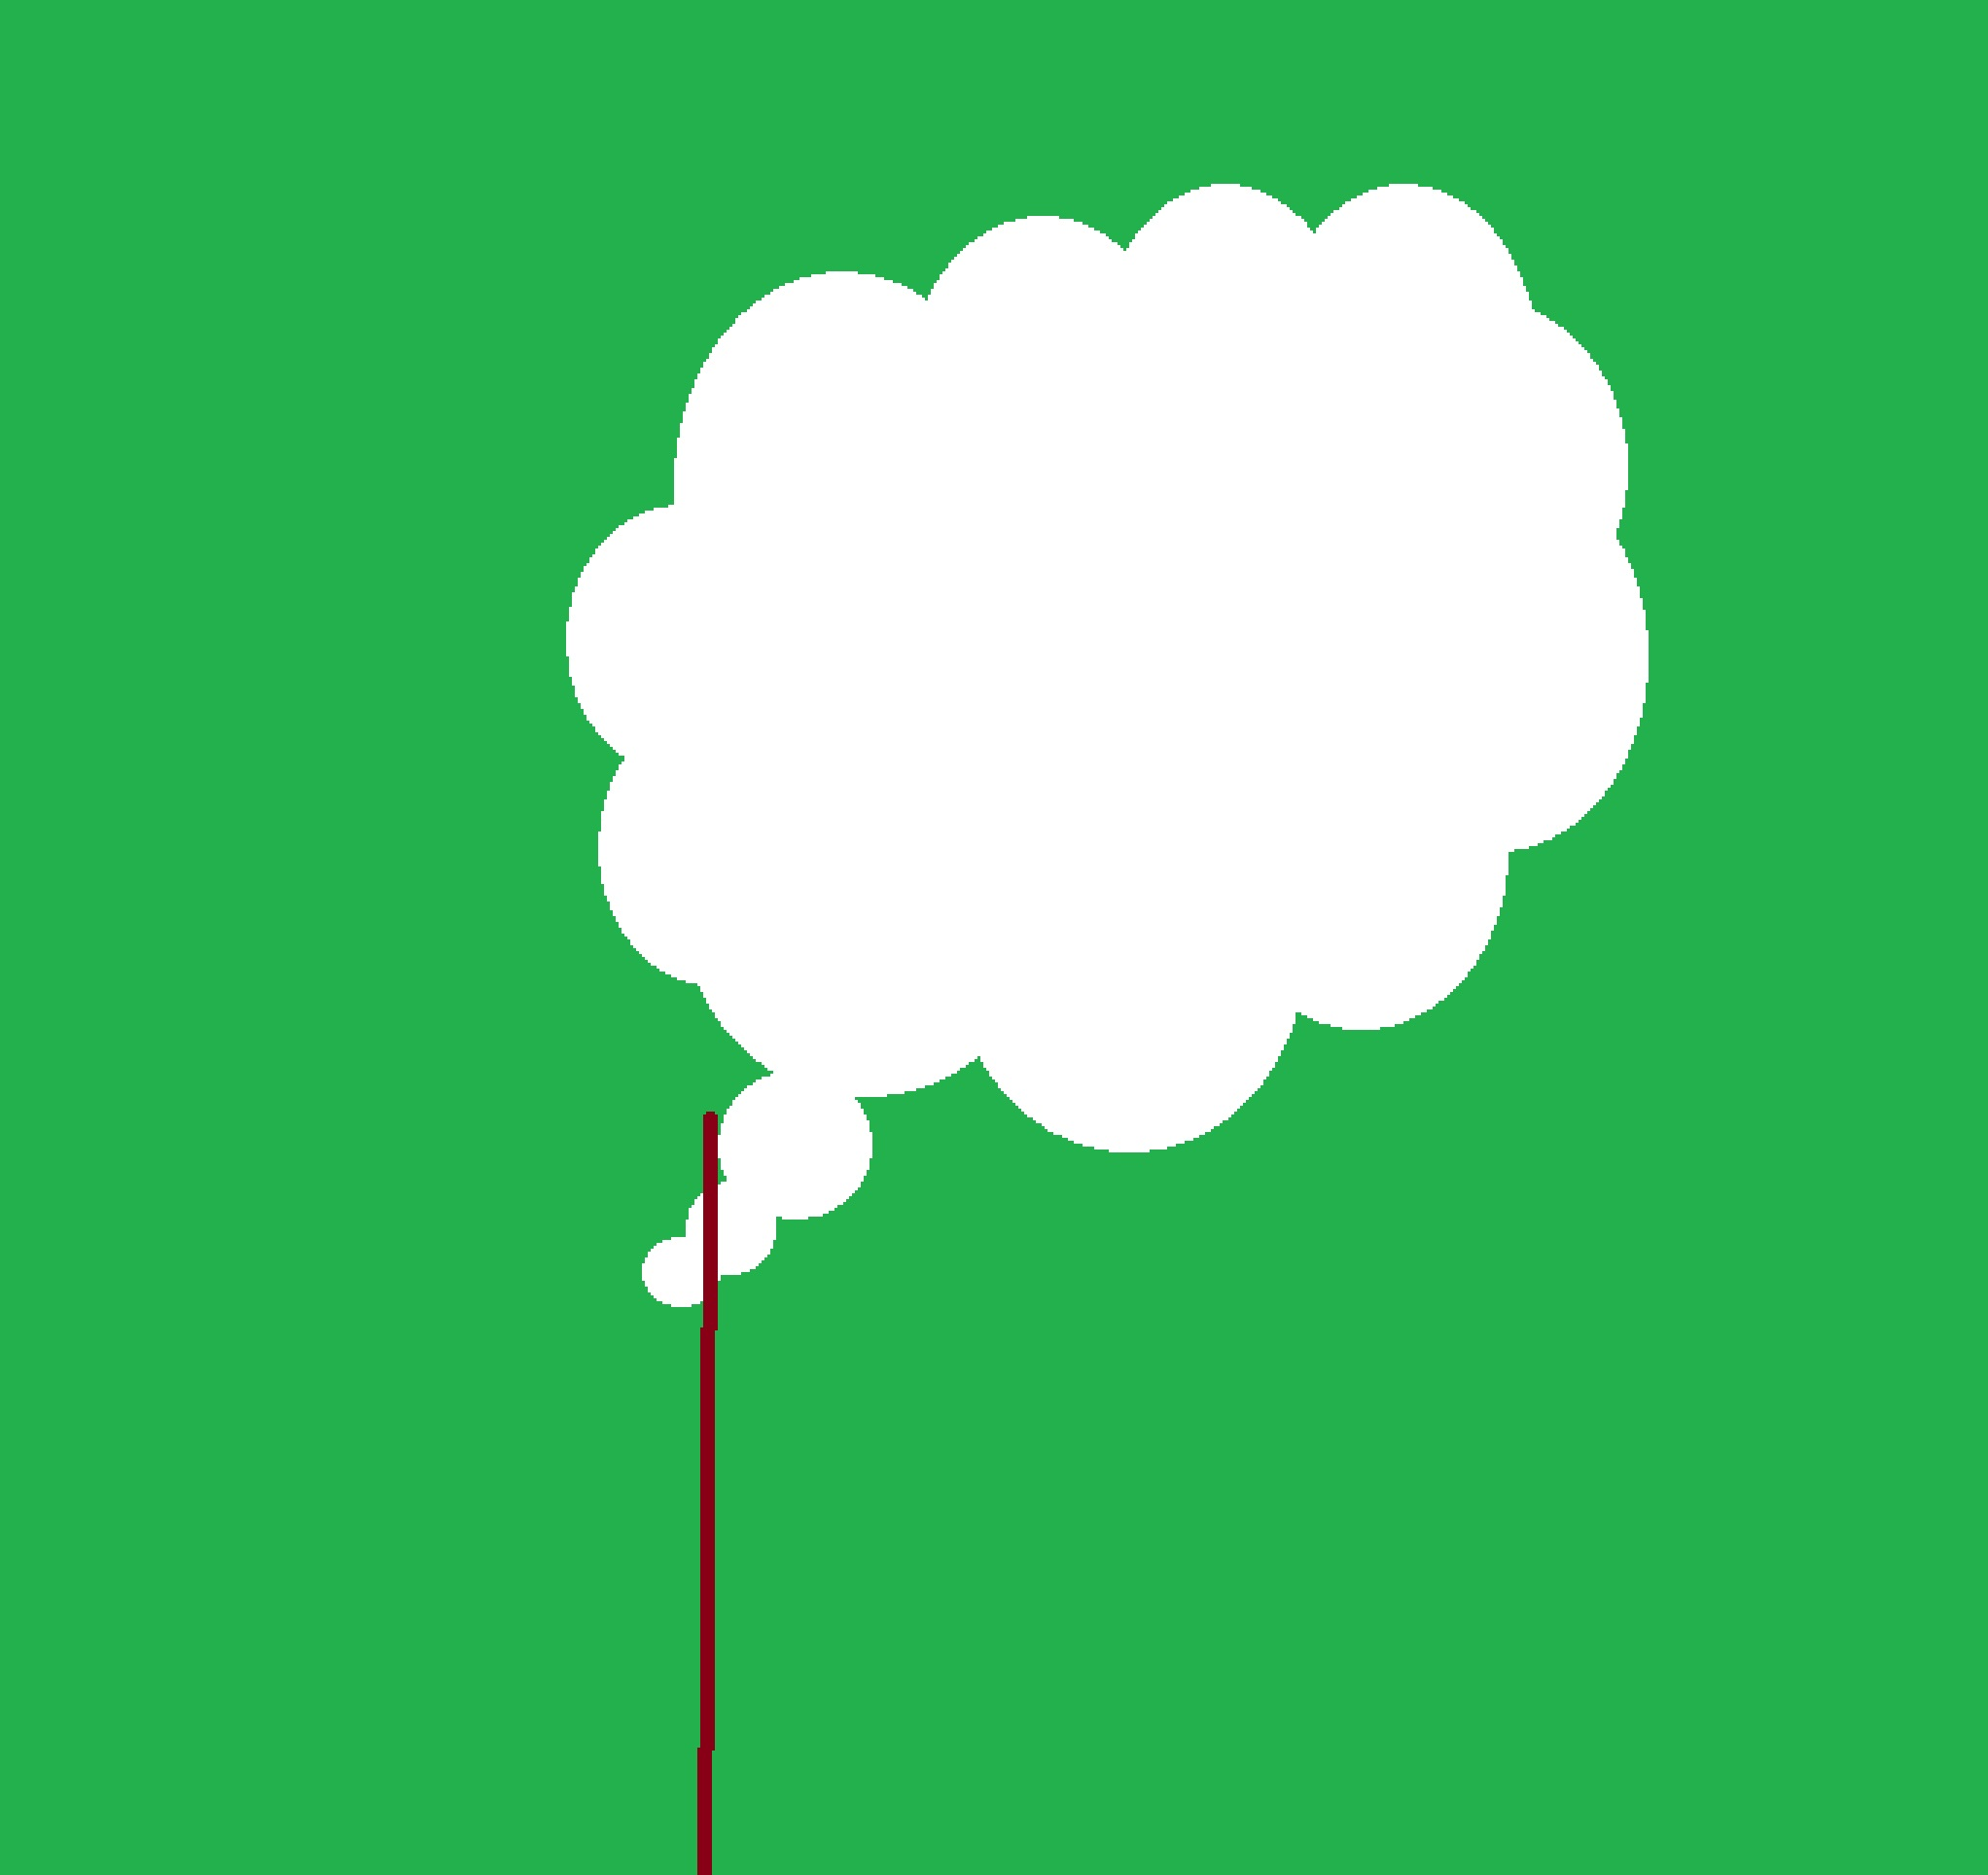
\includegraphics[height=3cm]{czosnek.jpg}
 \caption{Obraz numer 6}
 \label{figure:example5}
\end{figure}
W typologii siedlisk leśnych uznawany jest za gatunek charakterystyczny dla siedlisk lasu wilgotnego (Lw), lasu wyżynnego wilgotnego (Lwyżw) i lasu górskiego wilgotnego (LGw), pozwalający na odróżnienie ich od odpowiednich lasów świeżych.

Na Wyspach Brytyjskich gatunek ten jest jednym z indykatorów starych lasów (ang. ancient forests).

\subsection{Fitosocjologia}
W Polsce gatunek charakterystyczny dla rzędu (O.) Fagetalia, w Czechach dla podzwiązku Ulmenion. W Europie Środkowej, a także w Skandynawii, rośnie najczęściej w buczynach, zwłaszcza w żyznej buczynie niżowej, poza tym w niskich grądach, nadrzecznej olszynie górskiej i żyznej buczynie sudeckiej oraz w łęgach. W Europie Zachodniej podawany jest jako rosnący najczęściej w grądach z dębem szypułkowym Quercus robur i leszczyną Corylus avellana, w lasach z jesionem wyniosłym na głęboko próchnicznych i zasobnych glebach, a także łęgach z olszą czarną i zaroślach nadrzecznych. Niektóre źródła wskazują na niską wartość syntaksonomiczną czosnku niedźwiedziego i innych gatunków runa leśnego o podobnych wymaganiach ekologicznych tworzących grupę zwaną Corydalis. Rosną one bowiem w różnych zespołach leśnych, pod różnymi drzewostanami liściastymi, zawsze jednak wskazując na ich wariant bardzo żyzny i wilgotny, rozwijający się zwykle na glinach zasobnych w węglan wapnia (do grupy tej należą poza czosnkiem m.in. zawilec żółty, kokorycz pusta i pełna, złoć żółta i podagrycznik pospolity).

\begin{figure}
 \centering
 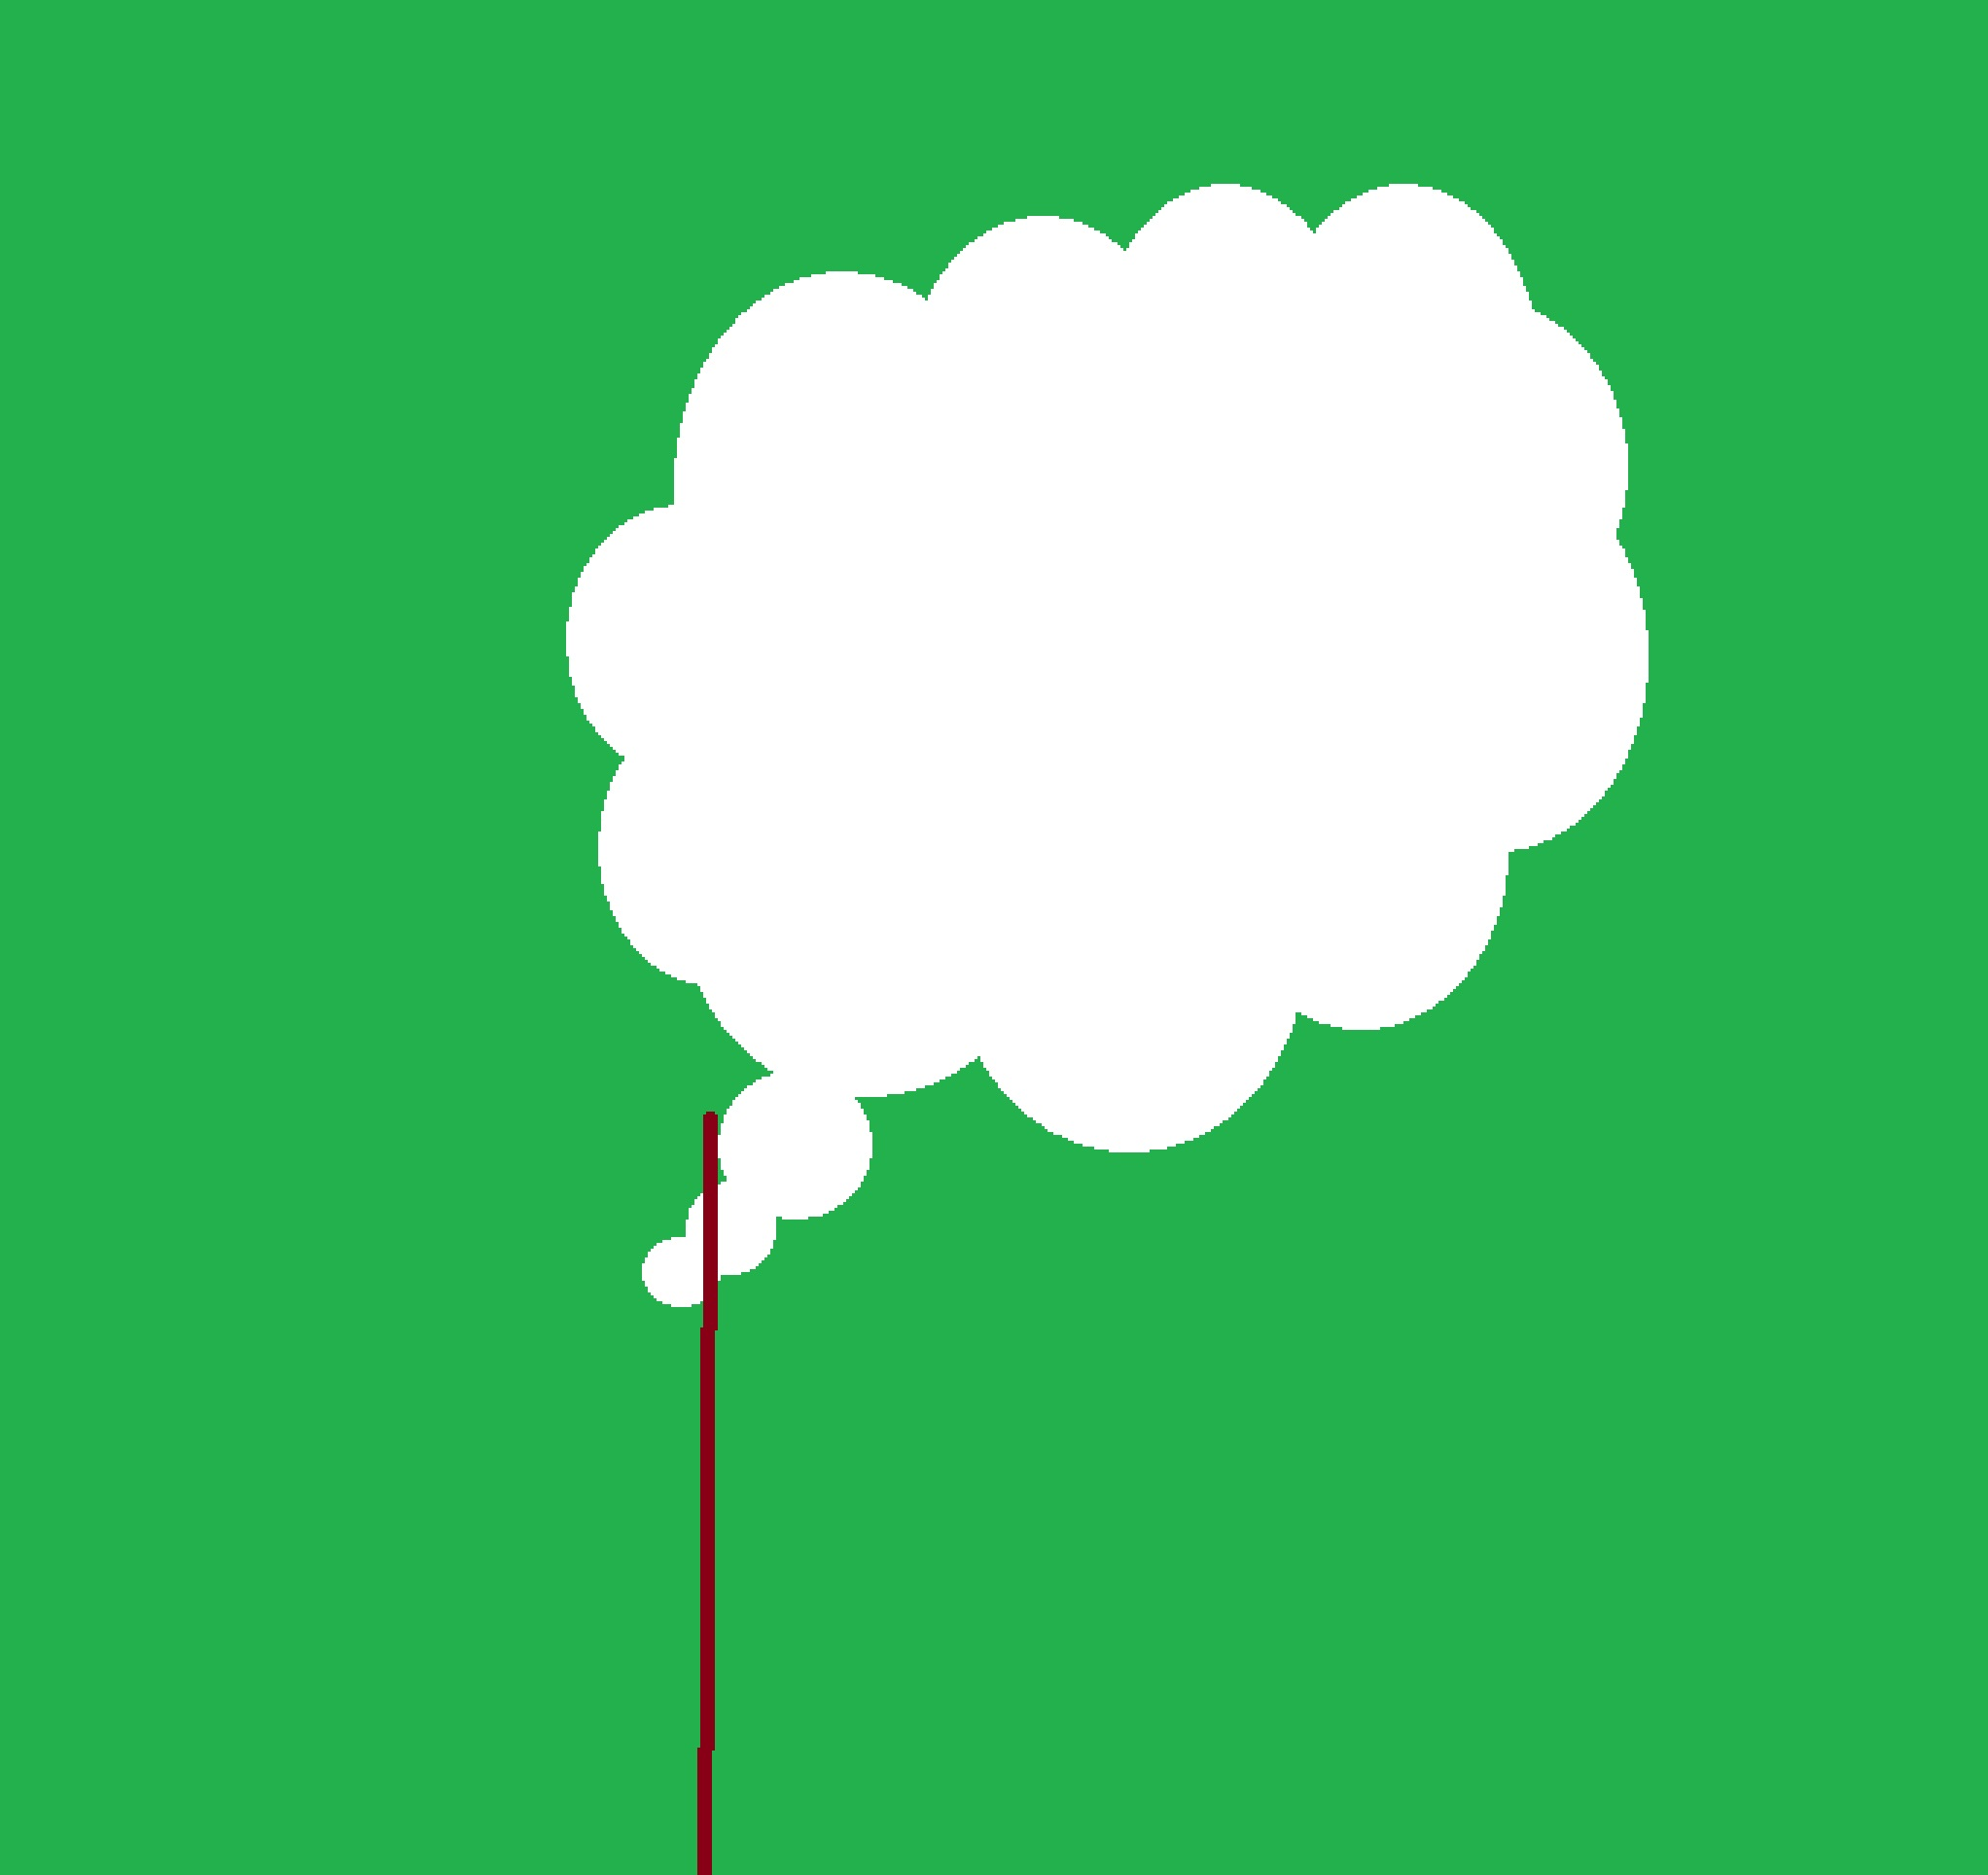
\includegraphics[height=3cm]{czosnek.jpg}
 \caption{Obraz numer 5}
 \label{figure:example6}
\end{figure}

\subsection{Oddziaływanie międzygatunkowe}
Czosnek niedźwiedzi bywa zgryzany przez bydło, natomiast nie jest zgryzany przez dziko żyjącą zwierzynę. Z gatunkiem tym związane są nieliczne roślinożerne bezkręgowce – Cheilosia maculata i Cheilosia fasciata. Z powodu krótkodystansowego rozprzestrzeniania nasion i w pewnym stopniu też dzięki rozmnażaniu wegetatywnemu, gatunek tworzy często zwarte i zwykle niemal jednogatunkowe łany. Masowe występowanie czosnku niedźwiedziego, powodującego zakrywanie gleby do połowy lata, skutkuje eliminacją gatunków konkurencyjnych (niektóre gatunki towarzyszące, jak przytulia wonna, utrzymują się rozrastając się w takich miejscach przez pozostałą część sezonu wegetacyjnego). Podobnie, ograniczając rozwój gatunków konkurencyjnych, działają także związki fenolowe wytwarzane do gleby przez czosnek niedźwiedzi (allelopatia). Stwierdzono, że olejek eteryczny czosnku silnie powstrzymuje kiełkowanie innych roślin. Nie stwierdzono jednak oddziaływania allelopatycznego w odniesieniu do takich gatunków jak szczyr trwały i bluszczyk kurdybanek.

\begin{figure}
 \centering
 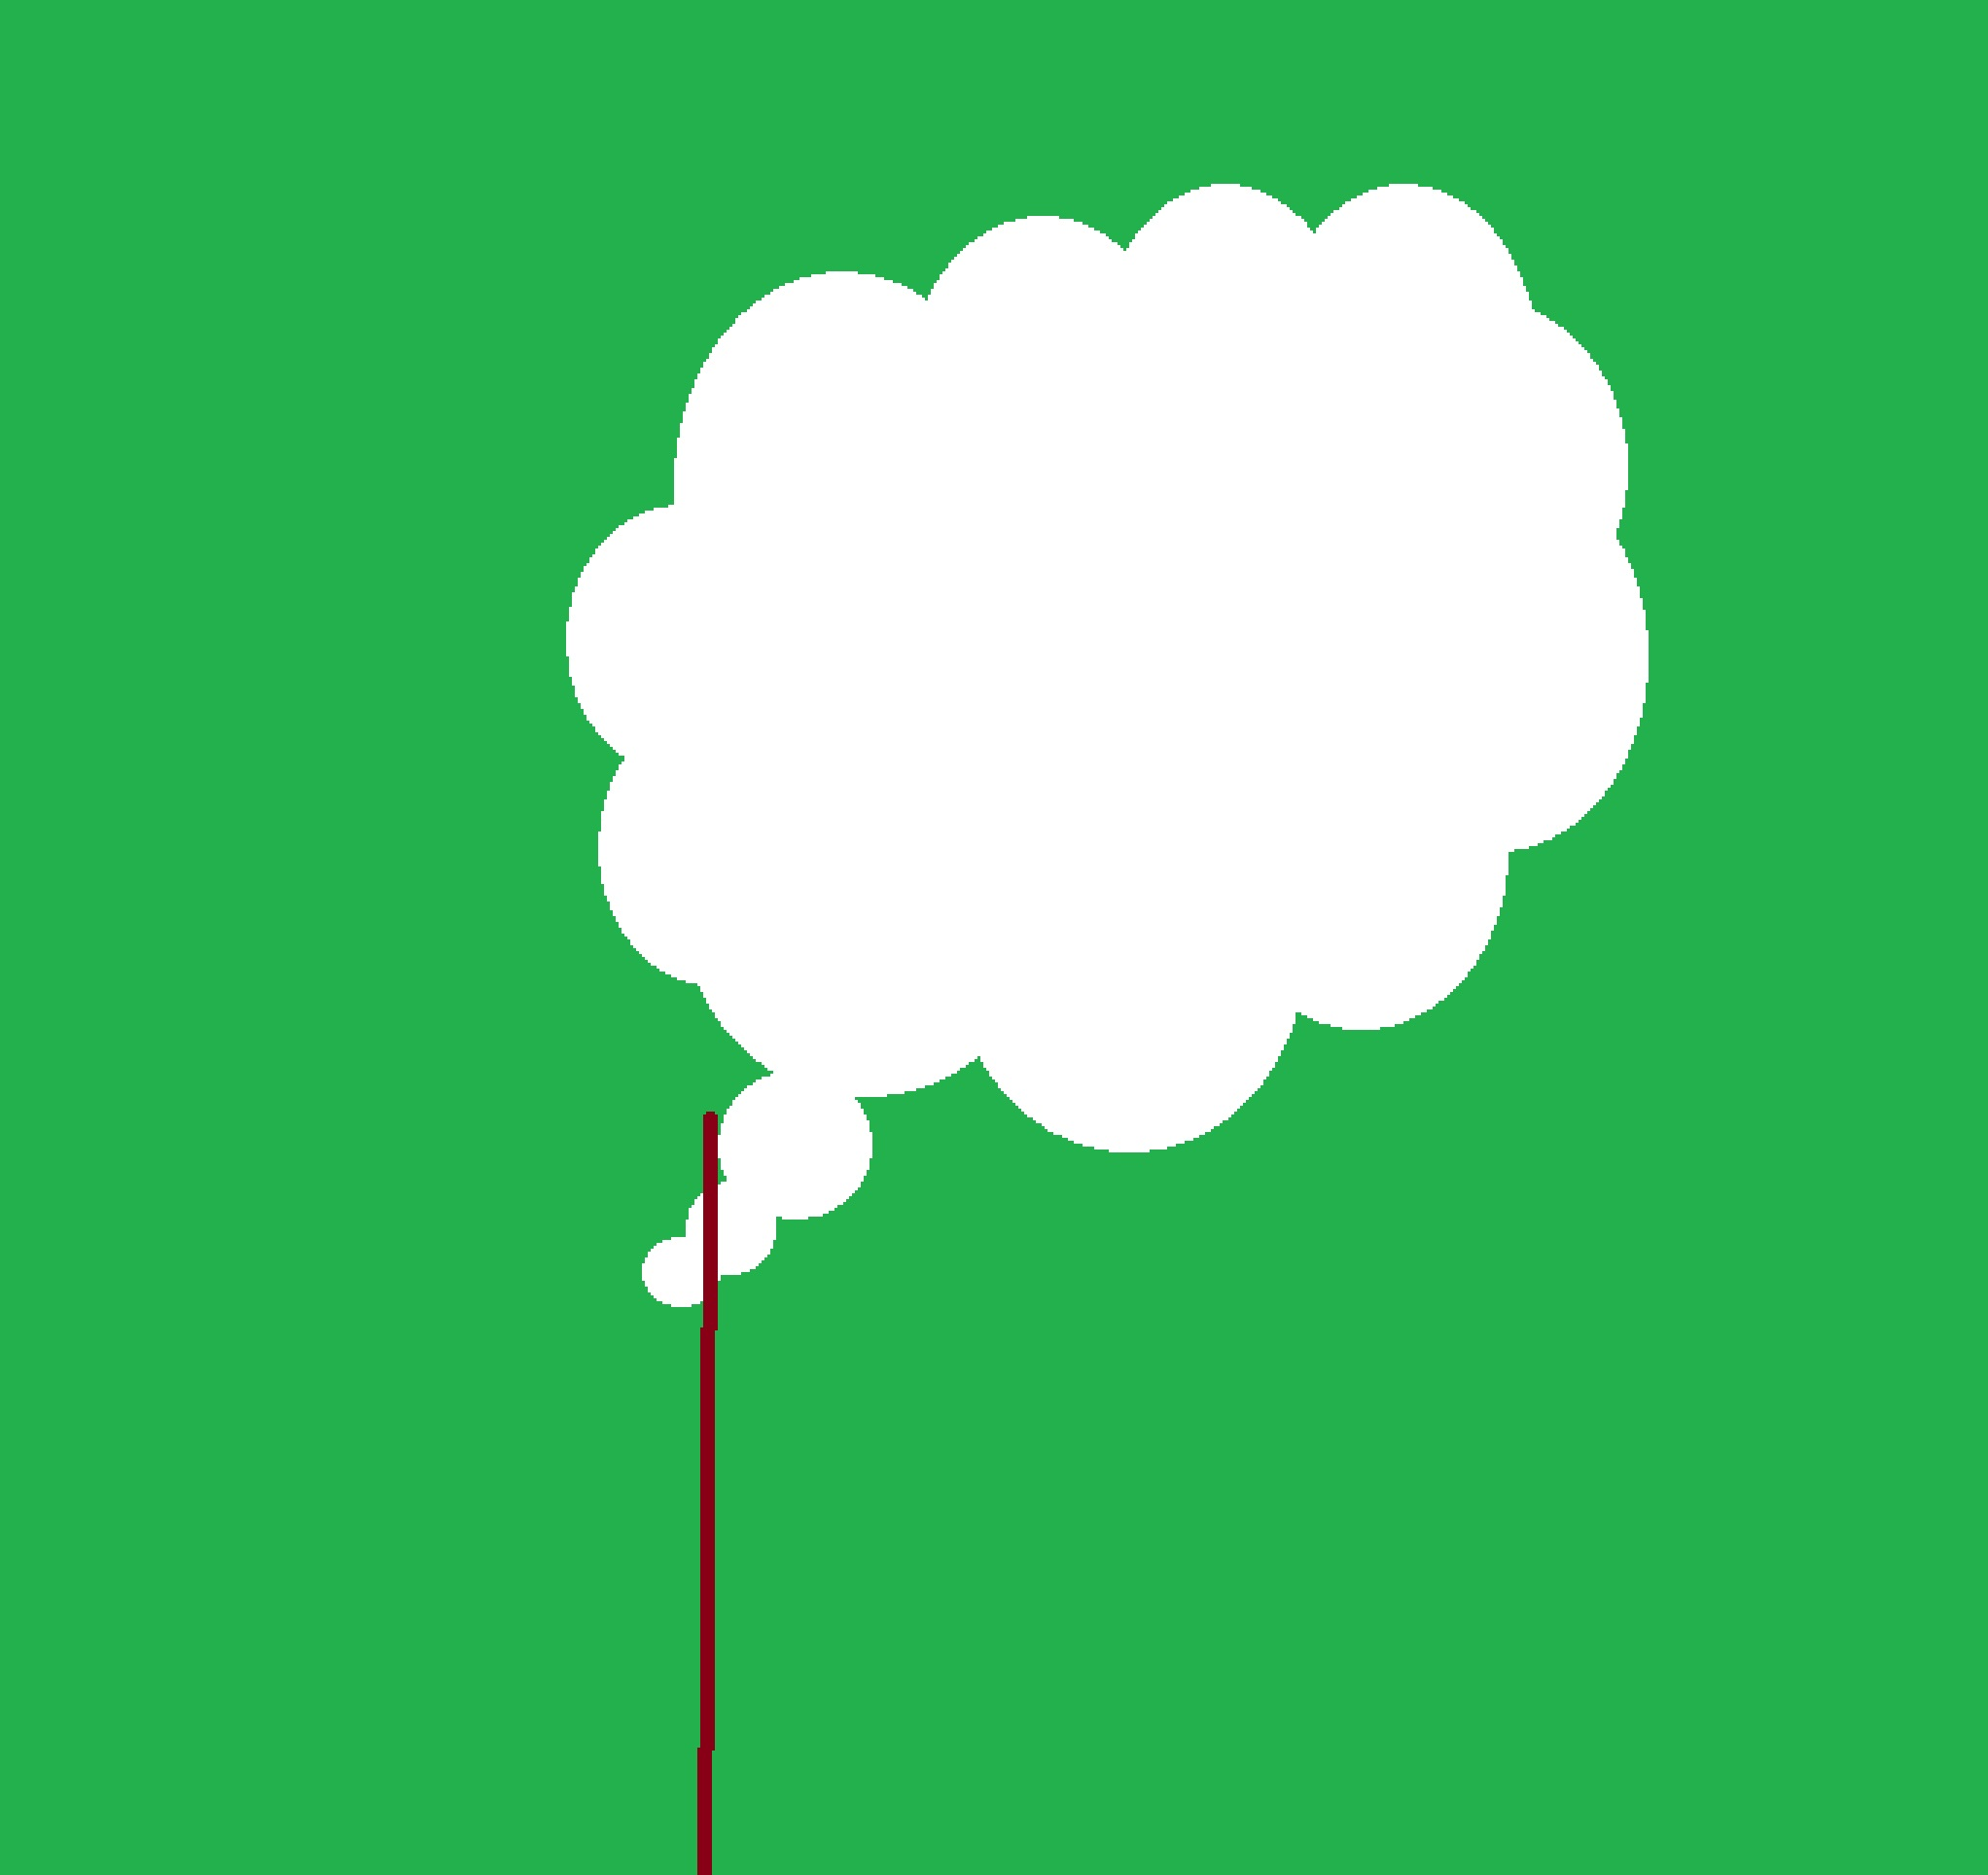
\includegraphics[height=3cm]{czosnek.jpg}
 \caption{Obraz numer 4}
 \label{Img1}
\end{figure}

Na stanowiskach czosnku niedźwiedziego zarejestrowano bogaty rozwój mezofauny glebowej, w szczególności skoczogonków. Zwierzęta te korzystają wczesnym latem z wielkiej ilości materii organicznej po obumarciu pędów nadziemnych czosnku, przyczyniając się wraz z mikroorganizmami do ich szybkiej mineralizacji.

Z korzeni czosnku wyizolowano mikoryzowy grzyb Pythium ultimum.

Do patogenów rzadko rejestrowanych na tym gatunku należy Botrytis allii, powodujący żółknięcie liści i zamieranie cebul. Z kolei infekcja Botrytis globosa objawia się ciemnozielonymi, zapadniętymi i
 wodnistymi plamami na liściach. Udokumentowano także na tym gatunku Sclerotina globosa.
